\documentclass[aspectratio=169]{beamer}
\usetheme{Madrid}
\usecolortheme{whale}
\usepackage{graphicx}
\usepackage{iftex}
% Helvetica Neue under XeLaTeX/LuaLaTeX when installed; TeX Gyre Heros (a
% Helvetica clone shipped with TeX Live) otherwise, and helvet under pdfLaTeX.
\ifPDFTeX
  \usepackage[utf8]{inputenc}
  \usepackage[T1]{fontenc}
  \usepackage[scaled]{helvet}
\else
  \usepackage{fontspec}
  \IfFontExistsTF{Helvetica Neue}{\setsansfont{Helvetica Neue}}{%
    \setsansfont{texgyreheros}[Extension=.otf, UprightFont=*-regular, BoldFont=*-bold,
      ItalicFont=*-italic, BoldItalicFont=*-bolditalic]}
\fi
\usepackage{array}
\usepackage{adjustbox}
\graphicspath{{../figures/}}
\setbeamertemplate{navigation symbols}{}
% No bottom bar: just "n / N" in the bottom-right corner.
\setbeamertemplate{footline}{%
  \hfill{\usebeamercolor[fg]{page number in head/foot}\usebeamerfont{page number in head/foot}%
  \insertframenumber\,/\,\inserttotalframenumber}\hspace*{2ex}\vskip4pt}
\setbeamerfont{frametitle}{size=\large}
% Deck section, bold caps, top-right of the title bar: \begin{frame}[category=Conferences]{...}.
% Reset before every frame so a category never carries over to the next slide.
\makeatletter
\def\slidecategory{}
\define@key{beamerframe}{category}{\def\slidecategory{#1}}
\AddToHook{env/frame/before}{\def\slidecategory{}}
\setbeamerfont{slide category}{size=\scriptsize,series=\bfseries}
\setbeamertemplate{frametitle}{%
  \nointerlineskip
  \begin{beamercolorbox}[wd=\paperwidth,leftskip=.3cm,rightskip=.3cm]{frametitle}%
    \vskip1pt
    \hbox to \dimexpr\paperwidth-.6cm\relax{\hfill\usebeamerfont{slide category}\strut\MakeUppercase{\slidecategory}}%
    \vskip-5pt
    \usebeamerfont{frametitle}\strut\insertframetitle\par
    \vskip1pt
  \end{beamercolorbox}}
\makeatother
\renewcommand{\arraystretch}{1.08}

\title[Radiology AI]{Artificial Intelligence in Pediatric Radiology}
\author{Joseph Rich, Dr.~Amit Sura}
\date{September 23, 2026}

\begin{document}

\frame{\titlepage}

\begin{frame}{Objectives}
\begin{itemize}
  \item Describe the big players in radiology AI, both general and pediatric, since 2023
  \item Summarize what radiology AI does well and what remains unresolved
\end{itemize}
\end{frame}

\begin{frame}{Methods}
\vspace{-4pt}
{\small
\textbf{Journals, Preprints}: PubMed, Embase, arXiv, medRxiv\\
\textbf{Conferences}: NeurIPS, ICLR, ICML, CVPR, MICCAI, MIDL\\
\textbf{Datasets}: Hand-curated list\\
\textbf{Newsletters}: The Imaging Wire, RSNA News, TLDR AI, TLDR Tech, Signify Research, ESR / ECR, Radiology Business\\
\textbf{Commercial}: FDA list of AI-enabled devices\par}
\vspace{2pt}
{\small\textbf{Search strategy}: radiology AND AI [AND pediatric]\par}
\vspace{2pt}
{\tiny\fontsize{6}{7.3}\selectfont\raggedright
\textbf{radiology}: (radiology[tiab] OR radiological[tiab] OR radiograph*[tiab] OR "medical imaging"[tiab] OR "diagnostic imaging"[tiab] OR tomography[tiab] OR "magnetic resonance"[tiab] OR MRI[tiab] OR "MR imaging"[tiab] OR "MR images"[tiab] OR MRIs[tiab] OR "MR image"[tiab] OR "MR scan"[tiab] OR "MR scans"[tiab] OR "computed tomography"[tiab] OR CT[tiab] OR ultrasound[tiab] OR ultrasonograph*[tiab] OR sonograph*[tiab] OR echocardiograph*[tiab] OR mammograph*[tiab] OR "chest x-ray"[tiab] OR "x-ray"[tiab] OR fluoroscop*[tiab] OR scintigraph*[tiab] OR "positron emission"[tiab] OR PET[tiab] OR SPECT[tiab] OR angiograph*[tiab] OR neuroimaging[tiab] OR tractograph*[tiab] OR elastograph*[tiab] OR "fMRI"[tiab] OR "functional MRI"[tiab] OR "functional magnetic resonance"[tiab] OR connectome*[tiab] OR "diffusion tensor"[tiab] OR DTI[tiab] OR "bone age"[tiab] OR "skeletal age"[tiab] OR "skeletal maturity"[tiab] OR "barium enema"[tiab])\\[2pt]
\textbf{AI}: ("artificial intelligence"[tiab] OR "machine learning"[tiab] OR "deep learning"[tiab] OR "convolutional neural network"[tiab] OR "convolutional neural networks"[tiab] OR "neural network"[tiab] OR "neural networks"[tiab] OR "computer-aided diagnosis"[tiab] OR "computer aided diagnosis"[tiab] OR "computer-aided detection"[tiab] OR radiomic*[tiab] OR "computer vision"[tiab] OR "large language model"[tiab] OR "large language models"[tiab] OR "foundation model"[tiab] OR "foundation models"[tiab] OR "transfer learning"[tiab] OR "vision transformer"[tiab] OR "self-supervised"[tiab] OR "random forest"[tiab] OR "support vector machine"[tiab] OR "gradient boosting"[tiab] OR "natural language processing"[tiab])\\[2pt]
\textbf{pediatric}: (pediatric*[tiab] OR paediatric*[tiab] OR child*[tiab] OR infant*[tiab] OR neonat*[tiab] OR adolescen*[tiab] OR fetal[tiab] OR foetal[tiab] OR fetus*[tiab] OR foetus*[tiab] OR newborn*[tiab] OR preterm[tiab] OR "premature infant"[tiab] OR "premature infants"[tiab] OR "premature birth"[tiab] OR "premature neonate"[tiab] OR "premature neonates"[tiab] OR prenatal[tiab] OR antenatal[tiab] OR perinatal[tiab] OR youth[tiab] OR juvenile[tiab] OR "children's hospital"[tiab] OR schoolchild*[tiab] OR toddler*[tiab])
\par}
\end{frame}

\begin{frame}[category=Journals]{Study selection}
\begin{center}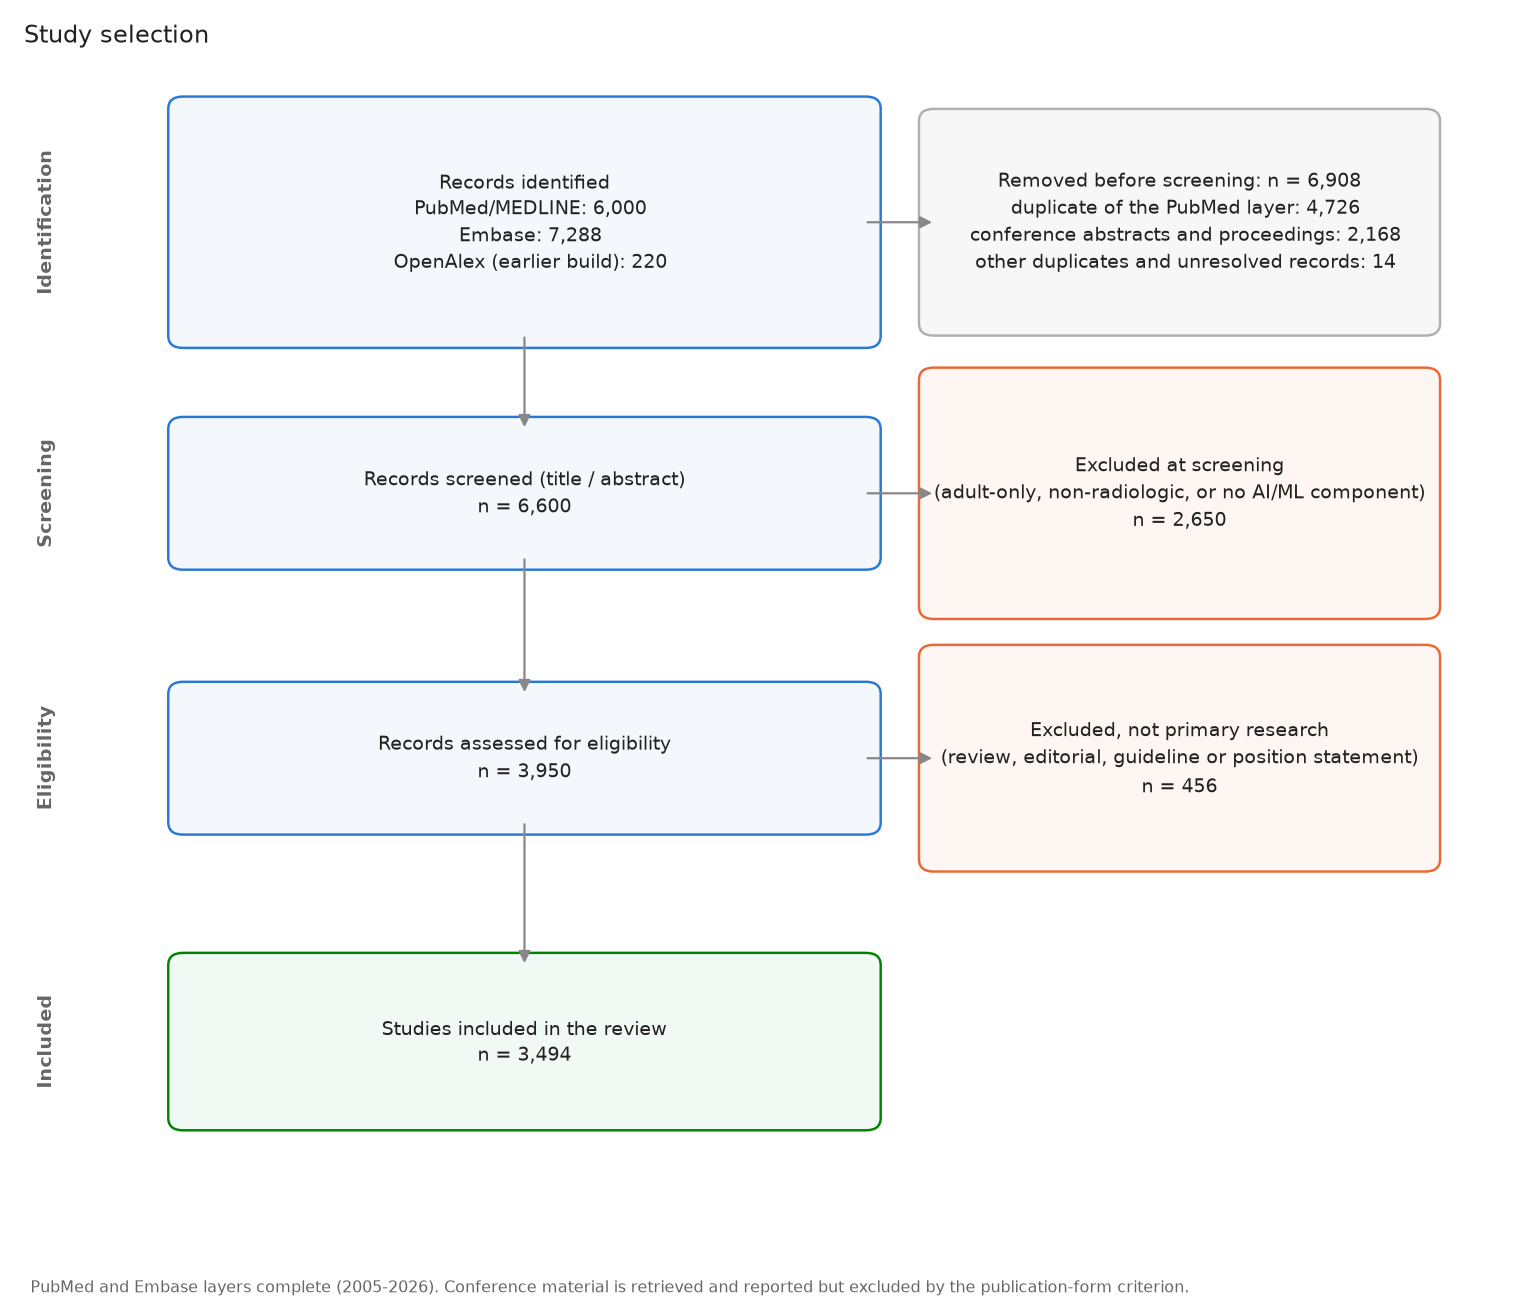
\includegraphics[height=0.76\textheight,width=\textwidth,keepaspectratio]{review_prisma.png}\end{center}
\end{frame}

\begin{frame}[category=Journals]{Radiology AI publication counts}
\begin{center}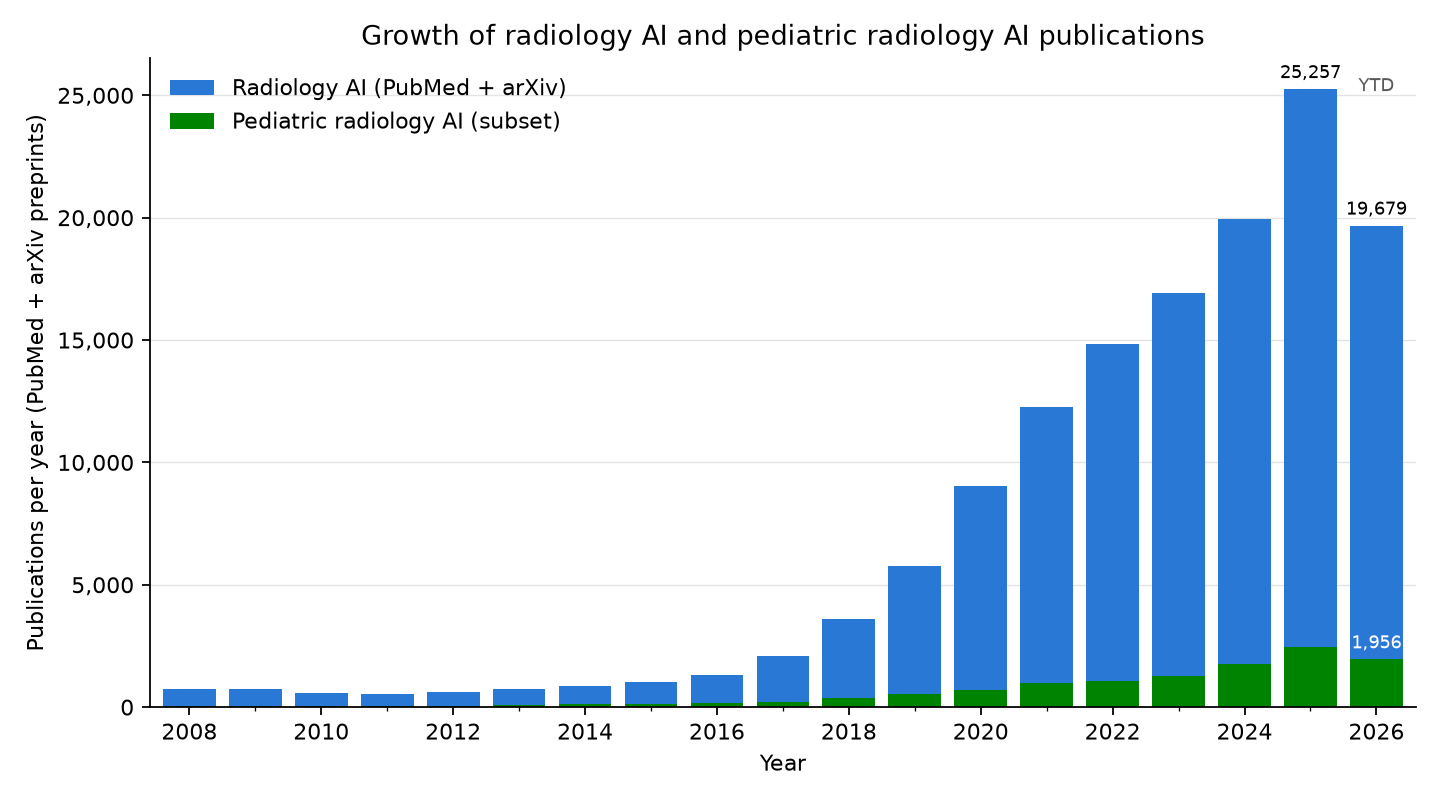
\includegraphics[height=0.80\textheight,width=\textwidth,keepaspectratio]{radiology_ai_trend.png}\end{center}
\end{frame}

\begin{frame}[category=Journals]{Which journals publish pediatric radiology AI}
\begin{center}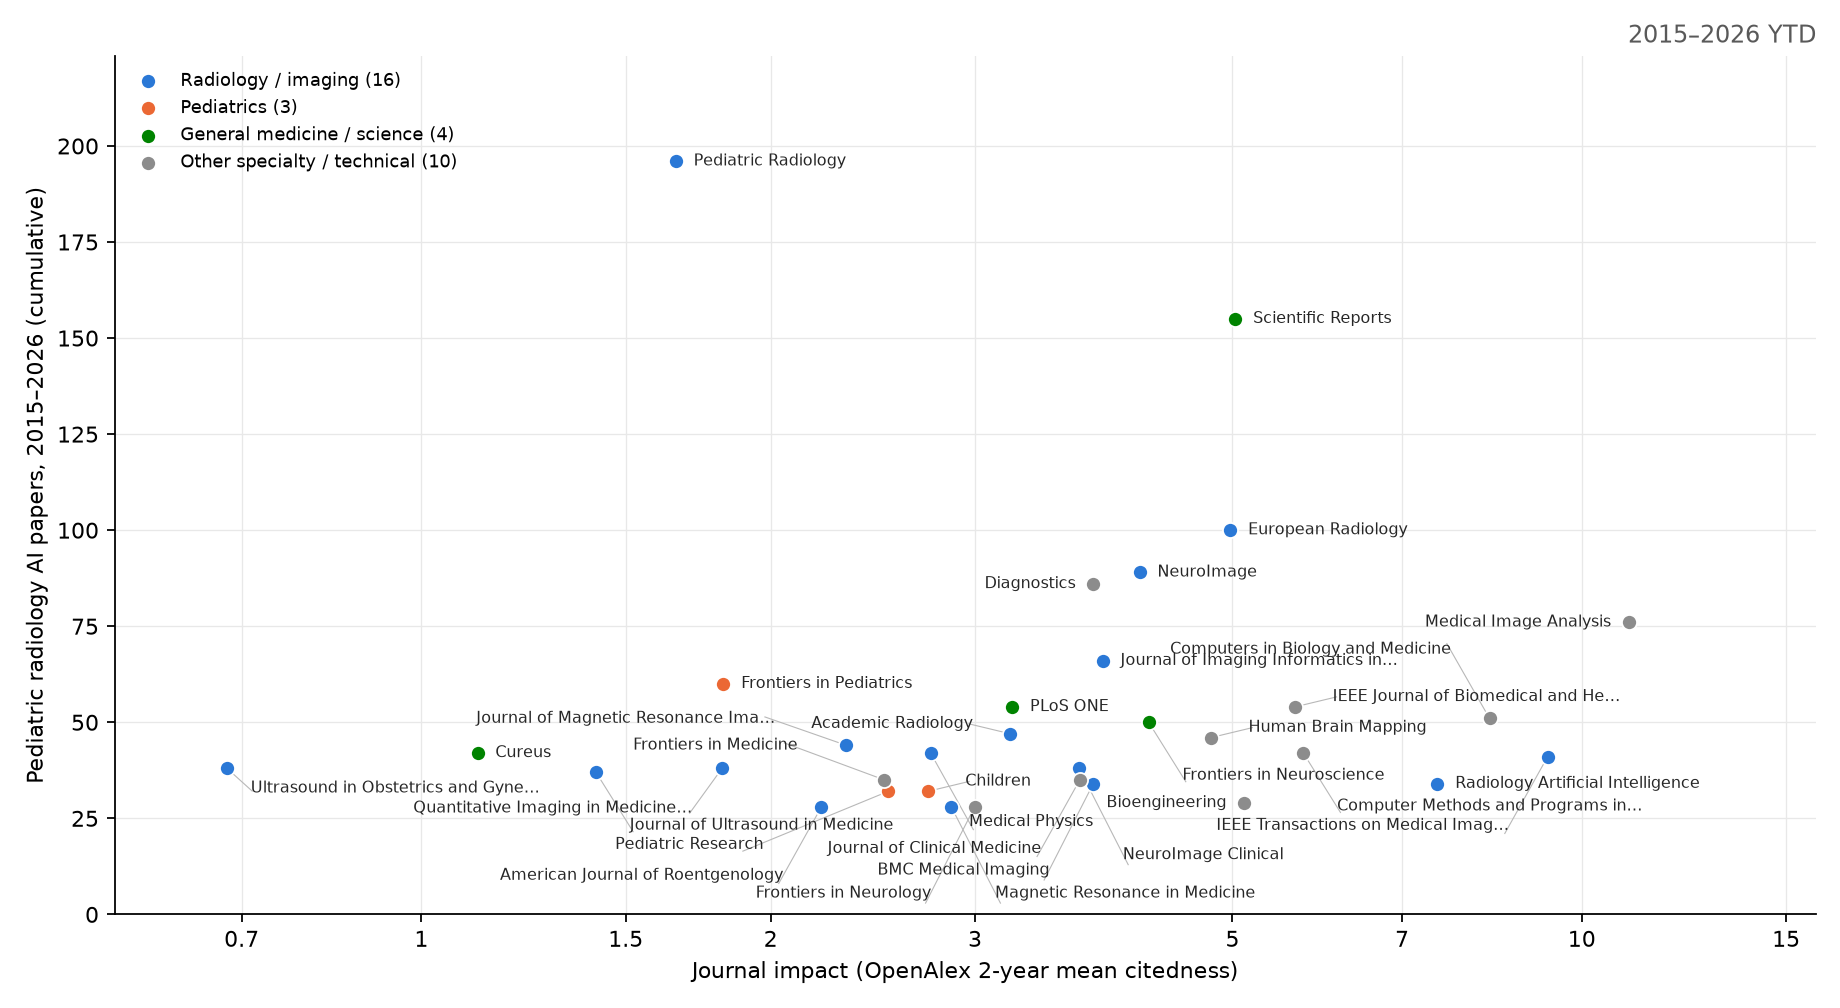
\includegraphics[height=0.66\textheight,width=\textwidth,keepaspectratio]{journal_impact.png}\end{center}
\vspace{-8pt}
{\tiny x = OpenAlex 2-year mean citedness (a free JIF analogue; runs below the published JIF). y = cumulative pediatric radiology-AI papers 2015-2026 (PubMed, strict title/abstract query). The 33 journals with at least 25 of them are shown, carrying 1,807 of 5,099; the rest is a long tail. Largest: Pediatric Radiology (196); median impact 3.7, 1 at 10 or above -- this work lands mostly in mid-impact specialty and technical journals. A further 3 conference proceedings and preprint servers clear the threshold (94 papers) but have no impact number of any kind and are not plotted. The same chart animated year by year: \texttt{figures/journal\_impact.gif}.}
\end{frame}

\begin{frame}[category=Journals]{Pediatric radiology AI publications, stratified by modality and task}
\begin{center}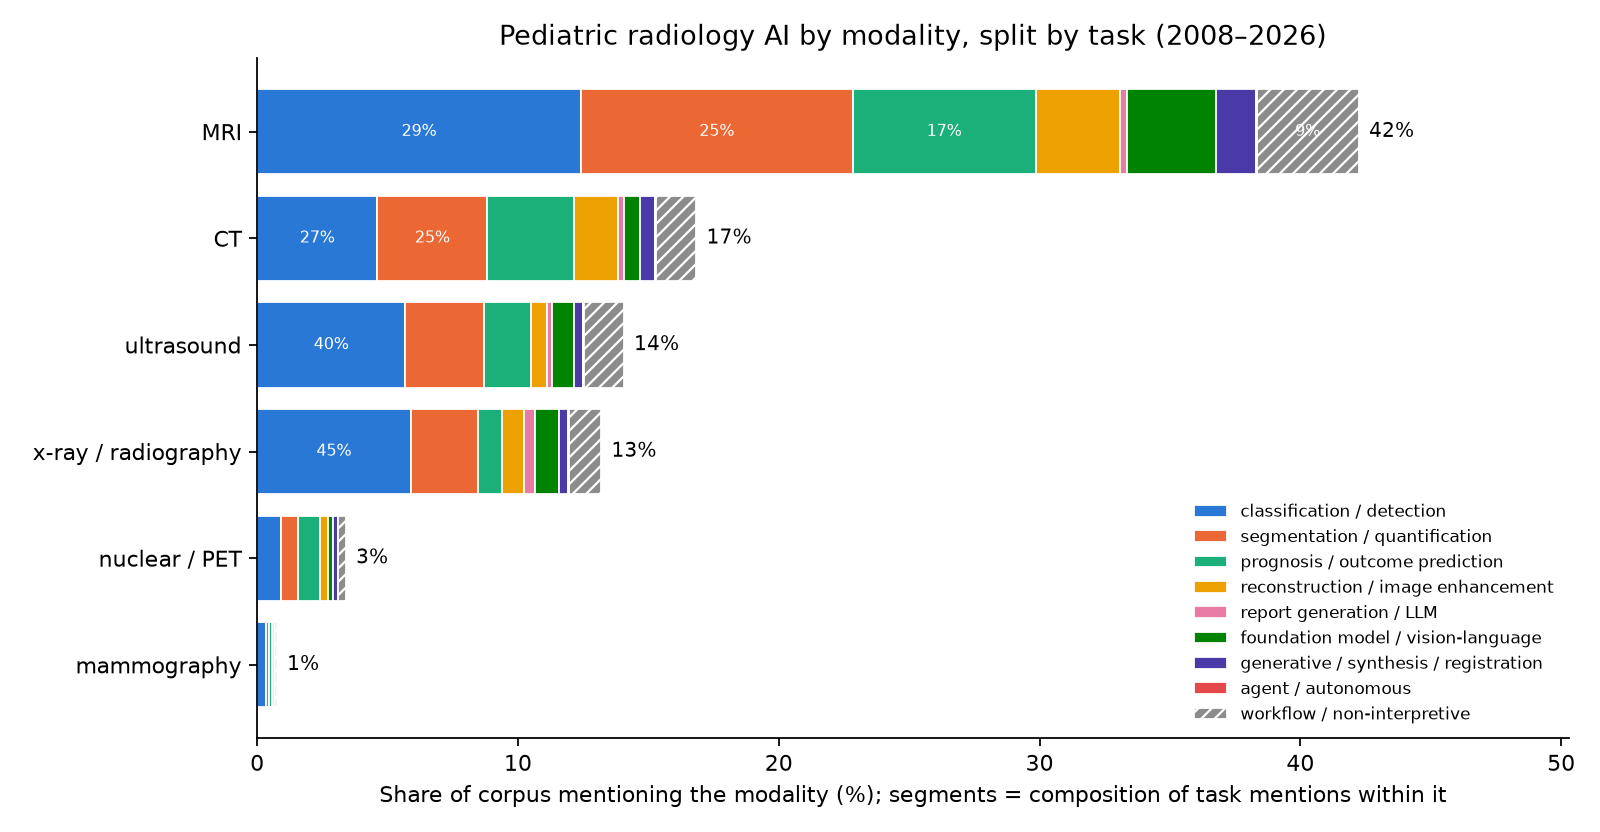
\includegraphics[height=0.47\textheight,width=\textwidth,keepaspectratio]{ped_modality_by_task.png}\end{center}
\vspace{-6pt}
{\tiny Same construction, restricted to the pediatric subset (10,737 papers incl. 596 preprints). Top pediatric modalities:
MRI 41\%, CT 16\%, ultrasound 13\%, x-ray / radiography 12\%. Mammography is omitted: its 79 pediatric-query hits (of 10,737) are adult breast-imaging papers whose abstracts mention children.}
\vspace{-2pt}
\tiny
\begin{columns}[T]
\begin{column}{0.33\textwidth}
\begin{itemize}
\item \textbf{detection / diagnosis}: is a finding present now, and which one (label or box): fracture, pneumonia, tumor; includes triage and screening
\item \textbf{segmentation}: outline a structure or lesion (a mask)
\item \textbf{measurement / quantification}: a number from the image: bone age, Cobb angle, organ volume, fetal biometry
\end{itemize}
\end{column}
\begin{column}{0.33\textwidth}
\begin{itemize}
\item \textbf{outcome prediction}: a future risk, response, or survival estimate from the image (prognosis, radiomics signatures)
\item \textbf{reconstruction / imputation}: a better or missing image: lower dose, faster scans, denoising, synthetic CT/MR
\item \textbf{report generation / LLM}: text: draft, summarize, or extract from radiology reports
\end{itemize}
\end{column}
\begin{column}{0.33\textwidth}
\begin{itemize}
\item \textbf{foundation model / vision-language}: a large pretrained model reused across tasks (segment-anything, self-supervised)
\item \textbf{agent / autonomous}: multi-step actions taken without a human in the loop
\item \textbf{workflow / non-interpretive}: protocoling, scheduling, ordering, decision support, education
\end{itemize}
\end{column}
\end{columns}
\end{frame}

\begin{frame}[category=Journals]{Pediatric radiology AI publications, stratified by medical problem}
\begin{center}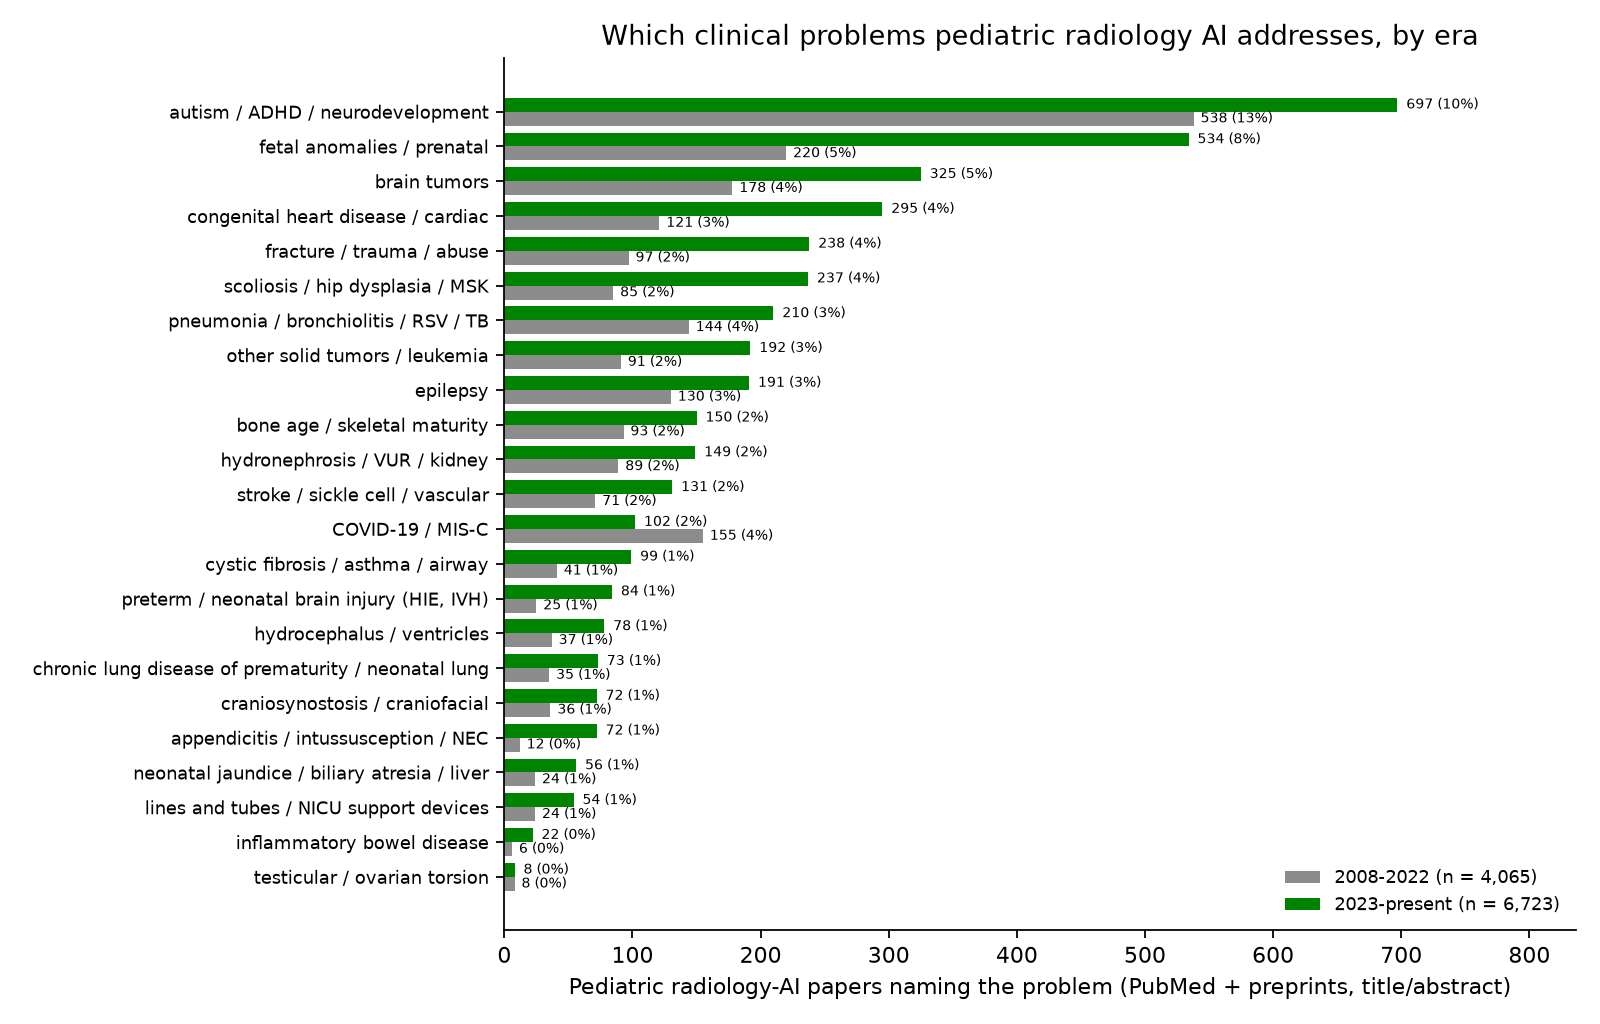
\includegraphics[height=0.82\textheight,width=\textwidth,keepaspectratio]{ped_problems.png}\end{center}
\end{frame}

\begin{frame}[category=Journals]{Most-cited radiology AI papers, 2008-2022}
\tiny
\begin{adjustbox}{max totalsize={\textwidth}{0.64\textheight}}
\renewcommand{\arraystretch}{1.2}
\begin{tabular}{|r|r|>{\raggedright\arraybackslash}p{0.459\textwidth}|>{\raggedright\arraybackslash}p{0.203\textwidth}|>{\raggedright\arraybackslash}p{0.338\textwidth}|}
\hline \textbf{Cites} & \textbf{FWCI} & \textbf{Paper} & \textbf{Venue} & \textbf{What it answers} \\ \hline
14,326 & 1023.0 & A survey on deep learning in medical image analysis (2017) & Medical Image Anal. & \textit{survey}: What can deep learning do across medical imaging? (the field's reference survey) \\ \hline
5,658 & 446.6 & Swin-Unet: Unet-like Pure Transformer for Medical Image Segmentation (2021) & ECCV Workshops & \textit{segmentation} \\ \hline
2,990 & 340.4 & Deep Learning in Medical Image Analysis (2017) & Annual Review of Biomedical Engineering & \textit{survey}: How does deep learning apply to medical image analysis? (review) \\ \hline
2,553 & 290.0 & Swin UNETR: Swin Transformers for Semantic Segmentation of Brain Tumors in MRI Images (2022) & BrainLes@MICCAI & \textit{segmentation} \\ \hline
2,769 & 272.4 & COVID-Net: a tailored deep convolutional neural network design for detection of COVID-19 cases from chest X-ray images (2020) & Scientific Reports & \textit{classification}: Can a CNN detect COVID-19 on chest X-ray? (COVID-Net) \\ \hline
3,634 & 236.9 & ChestX-Ray8: Hospital-Scale Chest X-Ray Database and Benchmarks on Weakly-Supervised Classification and Localization of Common Thorax Diseases (2017) & Computer Vision and Pattern Recognition & \textit{classification} \\ \hline
10,044 & 226.3 & nnU-Net: a self-configuring method for deep learning-based biomedical image segmentation (2020) & Nature Methods & \textit{segmentation}: Can one self-configuring method segment any organ or lesion without hand tuning? (nnU-Net) \\ \hline
4,100 & 170.2 & Convolutional neural networks: an overview and application in radiology (2018) & Insights into Imaging & \textit{tutorial}: What is a convolutional neural network, explained for radiologists? \\ \hline
5,587 & 158.4 & Computational Radiomics System to Decode the Radiographic Phenotype (2017) & Cancer Research & \textit{radiomics}: Can standardized image features (radiomics) be extracted reproducibly? (PyRadiomics) \\ \hline
3,322 & 149.0 & Artificial intelligence in radiology (2018) & Nature Reviews. Cancer & \textit{review}: How will AI change radiology practice? (Hosny et al.) \\ \hline
\end{tabular}
\end{adjustbox}
\\[1pt]
{\tiny FWCI = field-weighted citation impact (OpenAlex): citations relative to the world average for papers of the same field and year (1 = average)}
\end{frame}

\begin{frame}[category=Journals]{Most-cited radiology AI papers, 2023}
\tiny
\begin{adjustbox}{max totalsize={\textwidth}{0.64\textheight}}
\renewcommand{\arraystretch}{1.2}
\begin{tabular}{|r|r|>{\raggedright\arraybackslash}p{0.476\textwidth}|>{\raggedright\arraybackslash}p{0.210\textwidth}|>{\raggedright\arraybackslash}p{0.350\textwidth}|}
\hline \textbf{Cites} & \textbf{FWCI} & \textbf{Paper} & \textbf{Venue} & \textbf{What it answers} \\ \hline
1,608 & 615.8 & Segment anything in medical images & Nature Communications & \textit{foundation}: Can a prompt-based 'segment anything' model work on medical images? (MedSAM) \\ \hline
2,099 & 243.8 & Foundation models for generalist medical artificial intelligence & Nature & \textit{foundation model}: What would a single generalist medical AI model that handles images, text and records look like? (perspective) \\ \hline
702 & 118.5 & Redefining Radiology: A Review of Artificial Intelligence Integration in Medical Imaging & Diagnostics & \textit{survey / review}: Where does AI fit in radiology workflow, from acquisition to reporting? (review) \\ \hline
509 & 75.2 & Medical image analysis using deep learning algorithms & Frontiers in Public Health & \textit{other} \\ \hline
562 & 74.5 & A Study of CNN and Transfer Learning in Medical Imaging: Advantages, Challenges, Future Scope & Sustainability & \textit{other} \\ \hline
861 & 69.6 & Segment Anything Model for medical image analysis: an experimental study & Medical Image Anal. & \textit{segmentation}: How well does the unmodified Segment Anything Model work on medical images? (it needs prompts and adaptation) \\ \hline
573 & 55.8 & MRI-based brain tumor detection using convolutional deep learning methods and chosen machine learning techniques & BMC Medical Informatics and Decision Making & \textit{oncology} \\ \hline
460 & 44.5 & Brain Tumor Detection Based on Deep Learning Approaches and Magnetic Resonance Imaging & Cancers & \textit{oncology} \\ \hline
391 & 42.2 & SAM-Adapter: Adapting Segment Anything in Underperformed Scenes & 2023 IEEE/CVF International Conference on Computer Vision Workshops (ICCVW) & \textit{segmentation} \\ \hline
442 & 37.4 & A generalist vision--language foundation model for diverse biomedical tasks & Nature Medicine & \textit{other} \\ \hline
\end{tabular}
\end{adjustbox}
\\[1pt]
\end{frame}

\begin{frame}[category=Journals]{Most-cited radiology AI papers, 2024}
\tiny
\begin{adjustbox}{max totalsize={\textwidth}{0.64\textheight}}
\renewcommand{\arraystretch}{1.2}
\begin{tabular}{|r|r|>{\raggedright\arraybackslash}p{0.476\textwidth}|>{\raggedright\arraybackslash}p{0.210\textwidth}|>{\raggedright\arraybackslash}p{0.350\textwidth}|}
\hline \textbf{Cites} & \textbf{FWCI} & \textbf{Paper} & \textbf{Venue} & \textbf{What it answers} \\ \hline
1,074 & 225.2 & VM-UNet: Vision Mamba UNet for Medical Image Segmentation & ACM Transactions on Multimedia Computing, Communications, and Applications (TOMCCAP) & \textit{segmentation}: Does a state-space (Mamba) backbone beat convolutions and transformers for medical segmentation? \\ \hline
242 & 110.3 & Generalist foundation models from a multimodal dataset for 3D computed tomography & Nature Biomedical Engineering & \textit{other} \\ \hline
282 & 74.6 & Artificial intelligence in neuro-oncology: advances and challenges in brain tumor diagnosis, prognosis, and precision treatment & npj Precision Oncology & \textit{oncology} \\ \hline
279 & 72.6 & METhodological RadiomICs Score (METRICS): a quality scoring tool for radiomics research endorsed by EuSoMII & Insights into Imaging & \textit{radiomics}: How should the quality of a radiomics study be scored? (METRICS checklist) \\ \hline
349 & 47.6 & Deep learning for medical image segmentation: State-of-the-art advancements and challenges & Informatics in Medicine Unlocked & \textit{segmentation} \\ \hline
317 & 43.4 & Advances in Medical Image Segmentation: A Comprehensive Review of Traditional, Deep Learning and Hybrid Approaches & Bioengineering & \textit{segmentation} \\ \hline
238 & 37.0 & Employing deep learning and transfer learning for accurate brain tumor detection & Scientific Reports & \textit{oncology} \\ \hline
242 & 36.0 & Deep semi-supervised learning for medical image segmentation: A review & Expert systems with applications & \textit{segmentation} \\ \hline
241 & 34.5 & A review of deep learning-based information fusion techniques for multimodal medical image classification & Comput. Biol. Medicine & \textit{survey / review} \\ \hline
298 & 31.8 & Vision-language models for medical report generation and visual question answering: a review & Frontiers Artif. Intell. & \textit{report generation / LLM}: What can vision-language models do for report generation and visual question answering? (review) \\ \hline
\end{tabular}
\end{adjustbox}
\\[1pt]
{\tiny }
\end{frame}

\begin{frame}[category=Journals]{Most-cited radiology AI papers, 2025}
\tiny
\begin{adjustbox}{max totalsize={\textwidth}{0.64\textheight}}
\renewcommand{\arraystretch}{1.2}
\begin{tabular}{|r|r|>{\raggedright\arraybackslash}p{0.459\textwidth}|>{\raggedright\arraybackslash}p{0.203\textwidth}|>{\raggedright\arraybackslash}p{0.338\textwidth}|}
\hline \textbf{Cites} & \textbf{FWCI} & \textbf{Paper} & \textbf{Venue} & \textbf{What it answers} \\ \hline
258 & 225.8 & Deep Convolutional Neural Networks in Medical Image Analysis: A Review & Inf. & \textit{survey / review} \\ \hline
145 & 158.8 & Multi-model assurance analysis showing large language models are highly vulnerable to adversarial hallucination attacks during clinical decision support & Communications Medicine & \textit{LLM / reports} \\ \hline
122 & 108.2 & Multimodal generative AI for medical image interpretation & Nature & \textit{other} \\ \hline
313 & 94.9 & Towards generalist foundation model for radiology by leveraging web-scale 2D\&3D medical data & Nature Communications & \textit{foundation model}: Can a radiology foundation model trained on web-scale 2D and 3D scans generalize across modalities and tasks? (RadFM) \\ \hline
173 & 87.2 & Development and validation of an autonomous artificial intelligence agent for clinical decision-making in oncology & Nature Cancer & \textit{agent / autonomous}: Can an autonomous LLM agent that calls imaging and other tools support oncology decisions? (validation study) \\ \hline
208 & 65.9 & A review of deep learning for brain tumor analysis in MRI & npj Precision Oncology & \textit{survey / review} \\ \hline
150 & 65.8 & Med-R1: Reinforcement Learning for Generalizable Medical Reasoning in Vision-Language Models & IEEE Transactions on Medical Imaging & \textit{LLM / reports} \\ \hline
233 & 64.6 & Artificial intelligence in healthcare and medicine: clinical applications, therapeutic advances, and future perspectives & European Journal of Medical Research & \textit{other} \\ \hline
151 & 54.0 & Medical Image Segmentation: A Comprehensive Review of Deep Learning-Based Methods & Tomography & \textit{segmentation} \\ \hline
118 & 39.5 & Advanced Brain Tumor Classification in MR Images Using Transfer Learning and Pre-Trained Deep CNN Models & Cancers & \textit{oncology} \\ \hline
\end{tabular}
\end{adjustbox}
\\[1pt]
\end{frame}

\begin{frame}[category=Journals]{Most-cited radiology AI papers, 2026 (year to date)}
\tiny
\begin{adjustbox}{max totalsize={\textwidth}{0.64\textheight}}
\renewcommand{\arraystretch}{1.2}
\begin{tabular}{|r|r|>{\raggedright\arraybackslash}p{0.459\textwidth}|>{\raggedright\arraybackslash}p{0.203\textwidth}|>{\raggedright\arraybackslash}p{0.338\textwidth}|}
\hline \textbf{Cites} & \textbf{FWCI} & \textbf{Paper} & \textbf{Venue} & \textbf{What it answers} \\ \hline
48 & 102.6 & A generalizable foundation model for analysis of human brain MRI & Nature Neuroscience & \textit{other} \\ \hline
16 & 90.5 & Reporting checklist for foundation and large language models in medical research (REFINE): an international consensus guideline. & Diagnostic and Interventional Radiology & \textit{LLM / reports} \\ \hline
15 & 76.1 & Scaling medical AI across clinical contexts & Nature Medicine & \textit{foundation model}: How can medical AI be scaled across hospitals, populations and tasks without breaking? (perspective) \\ \hline
27 & 67.3 & Applications and limitations of large language models to integrate medical context: a comprehensive review & Iran Journal of Computer Science & \textit{survey / review} \\ \hline
18 & 62.7 & A hybrid deep learning framework based on VGG19 and U-Net for accurate brain tumor segmentation in MRI images & Magnetic Resonance Letters & \textit{segmentation} \\ \hline
37 & 58.8 & Explainable artificial intelligence (XAI) in medical imaging: a systematic review of techniques, applications, and challenges & BMC Medical Imaging & \textit{survey / review}: Which explainability methods are used in medical imaging AI and do they help? (review) \\ \hline
12 & 45.3 & Explainable AI-driven MRI-based brain tumor classification: a novel deep learning approach & Frontiers Artif. Intell. & \textit{oncology} \\ \hline
21 & 44.2 & Agentic AI in Radiology: Evolution from Large Language Models to Future Clinical Integration. & Radiology: Artificial Intelligence & \textit{agent / autonomous}: What are agentic AI systems in radiology and what stands between them and clinical use? (review) \\ \hline
17 & 28.4 & Leveraging multi-modal foundation models for analysing spatial multi-omic and histopathology data & Nature Biomedical Engineering & \textit{other} \\ \hline
19 & 21.4 & BIBSNet: A deep learning baby image brain segmentation network for MRI scans & Developmental Cognitive Neuroscience & \textit{segmentation}: Can one network segment infant brain MRI across the first years of life? (BIBSNet) \\ \hline
\end{tabular}
\end{adjustbox}
\\[1pt]
\end{frame}

\begin{frame}[category=Journals]{Most-cited pediatric radiology AI papers, 2008-2022}
\tiny
\begin{adjustbox}{max totalsize={\textwidth}{0.64\textheight}}
\renewcommand{\arraystretch}{1.2}
\begin{tabular}{|r|r|>{\raggedright\arraybackslash}p{0.459\textwidth}|>{\raggedright\arraybackslash}p{0.203\textwidth}|>{\raggedright\arraybackslash}p{0.338\textwidth}|}
\hline \textbf{Cites} & \textbf{FWCI} & \textbf{Paper} & \textbf{Venue} & \textbf{What it answers} \\ \hline
426 & 328.6 & Performance of a Deep-Learning Neural Network Model in Assessing Skeletal Maturity on Pediatric Hand Radiographs. (2017) & Radiology & \textit{bone age}: Can a CNN assess skeletal maturity as accurately as radiologists? \\ \hline
431 & 321.5 & Fully Automated Deep Learning System for Bone Age Assessment (2017) & Journal of digital imaging & \textit{bone age}: Fully automated bone age from hand radiographs \\ \hline
403 & 221.2 & Deep learning for automated skeletal bone age assessment in X-ray images (2017) & Medical Image Anal. & \textit{bone age}: Deep learning for automated bone age (BoNet) \\ \hline
143 & 73.0 & Computerized Bone Age Estimation Using Deep Learning Based Program: Evaluation of the Accuracy and Efficiency. (2017) & AJR. American journal of roentgenology & \textit{bone age}: Is a commercial deep-learning bone-age program accurate and faster in practice? \\ \hline
191 & 57.8 & A Review on Deep-Learning Algorithms for Fetal Ultrasound-Image Analysis (2022) & Medical Image Anal. & \textit{survey / review} \\ \hline
352 & 57.4 & Standard Plane Localization in Fetal Ultrasound via Domain Transferred Deep Neural Networks (2015) & IEEE journal of biomedical and health informatics & \textit{fetal MRI} \\ \hline
194 & 57.0 & Automatic Fetal Ultrasound Standard Plane Recognition Based on Deep Learning and IIoT (2021) & IEEE Transactions on Industrial Informatics & \textit{fetal MRI} \\ \hline
233 & 30.3 & Evaluation of deep convolutional neural networks for automatic classification of common maternal fetal ultrasound planes (2020) & Scientific Reports & \textit{fetal MRI} \\ \hline
458 & 27.0 & The RSNA Pediatric Bone Age Machine Learning Challenge. (2019) & Radiology & \textit{bone age}: How well can crowdsourced AI estimate bone age? (RSNA challenge, 260 teams) \\ \hline
253 & 25.8 & An ensemble of neural networks provides expert-level prenatal detection of complex congenital heart disease (2021) & Nature Medicine & \textit{detection} \\ \hline
\end{tabular}
\end{adjustbox}
\\[2pt]
{\tiny A different corpus from the systematic-review tables earlier in the deck: this is a citation search of
Semantic Scholar over radiology AI with a pediatric title filter, so it includes conference papers and is not
screened for eligibility. The review tables rank the screened corpus. Both are shown because neither contains
the other.}
\end{frame}

\begin{frame}[category=Journals]{Most-cited pediatric radiology AI papers, 2023}
\tiny
\begin{adjustbox}{max totalsize={\textwidth}{0.64\textheight}}
\renewcommand{\arraystretch}{1.2}
\begin{tabular}{|r|r|>{\raggedright\arraybackslash}p{0.510\textwidth}|>{\raggedright\arraybackslash}p{0.225\textwidth}|>{\raggedright\arraybackslash}p{0.375\textwidth}|}
\hline \textbf{Cites} & \textbf{FWCI} & \textbf{Paper} & \textbf{Venue} & \textbf{What it answers} \\ \hline
32 & 36.6 & Bone Age Assessment Using Artificial Intelligence in Korean Pediatric Population: A Comparison of Deep-Learning Models Trained With Healthy Chronological and Greulich-Pyle Ages as Labels & Korean Journal of Radiology & \textit{bone age} \\ \hline
62 & 33.6 & Standard fetal ultrasound plane classification based on stacked ensemble of deep learning models & Expert systems with applications & \textit{fetal ultrasound}: Can an ensemble of networks classify the standard fetal ultrasound planes? \\ \hline
27 & 33.5 & Bone age assessment based on deep neural networks with annotation-free cascaded critical bone region extraction & Frontiers in Artificial Intelligence & \textit{bone age} \\ \hline
43 & 23.8 & Review on deep learning fetal brain segmentation from Magnetic Resonance images & Artif. Intell. Medicine & \textit{segmentation} \\ \hline
37 & 20.2 & Transfer learning for accurate fetal organ classification from ultrasound images: a potential tool for maternal healthcare providers & Scientific Reports & \textit{fetal MRI} \\ \hline
34 & 16.6 & Deep Learning-Based Multiclass Brain Tissue Segmentation in Fetal MRIs & Italian National Conference on Sensors & \textit{segmentation} \\ \hline
43 & 9.7 & Deeplasia: deep learning for bone age assessment validated on skeletal dysplasias & Pediatric Radiology & \textit{bone age} \\ \hline
30 & 7.8 & Deep learning for estimation of fetal weight throughout the pregnancy from fetal abdominal ultrasound. & American Journal of Obstetrics \& Gynecology MFM & \textit{fetal MRI} \\ \hline
38 & 7.3 & Deep learning model for prenatal congenital heart disease (CHD) screening can be applied to retrospective imaging from the community setting, outperforming initial clinical detection in a well-annotated cohort & Ultrasound in Obstetrics and Gynecology & \textit{fetal ultrasound}: Does a prenatal congenital heart disease screening model work on retrospective real-world scans? \\ \hline
31 & 5.8 & MRI-Based End-To-End Pediatric Low-Grade Glioma Segmentation and Classification & Canadian Association of Radiologists journal = Journal l'Association canadienne des radiologistes & \textit{segmentation} \\ \hline
\end{tabular}
\end{adjustbox}
\\[1pt]
\end{frame}

\begin{frame}[category=Journals]{Most-cited pediatric radiology AI papers, 2024}
\tiny
\begin{adjustbox}{max totalsize={\textwidth}{0.64\textheight}}
\renewcommand{\arraystretch}{1.2}
\begin{tabular}{|r|r|>{\raggedright\arraybackslash}p{0.493\textwidth}|>{\raggedright\arraybackslash}p{0.217\textwidth}|>{\raggedright\arraybackslash}p{0.362\textwidth}|}
\hline \textbf{Cites} & \textbf{FWCI} & \textbf{Paper} & \textbf{Venue} & \textbf{What it answers} \\ \hline
17 & 34.8 & Intrapartum Ultrasound Image Segmentation of Pubic Symphysis and Fetal Head Using Dual Student-Teacher Framework with CNN-ViT Collaborative Learning & International Conference on Medical Image Computing and Computer-Assisted Intervention & \textit{segmentation} \\ \hline
30 & 23.8 & FetalBrainAwareNet: Bridging GANs with anatomical insight for fetal ultrasound brain plane synthesis & Comput. Medical Imaging Graph. & \textit{fetal MRI} \\ \hline
20 & 19.5 & Artificial intelligence assisted common maternal fetal planes prediction from ultrasound images based on information fusion of customized convolutional neural networks & Frontiers in Medicine & \textit{fetal MRI} \\ \hline
18 & 15.9 & Deep learning denoising reconstruction for improved image quality in fetal cardiac cine MRI & Frontiers in Cardiovascular Medicine & \textit{reconstruction}: Does deep-learning denoising improve fetal cardiac cine MRI? \\ \hline
30 & 15.1 & RTSeg-net: A lightweight network for real-time segmentation of fetal head and pubic symphysis from intrapartum ultrasound images & Comput. Biol. Medicine & \textit{segmentation} \\ \hline
16 & 13.4 & FetSAM: Advanced Segmentation Techniques for Fetal Head Biometrics in Ultrasound Imagery & IEEE Open Journal of Engineering in Medicine and Biology & \textit{segmentation} \\ \hline
23 & 7.0 & Deep learning-based automated lesion segmentation on pediatric focal cortical dysplasia II preoperative MRI: a reliable approach & Insights into Imaging & \textit{epilepsy}: Can focal cortical dysplasia lesions be found automatically on preoperative pediatric MRI? \\ \hline
18 & 5.3 & Integration of a Deep Convolutional Neural Network With Adaptive Channel Weight Technique for Automated Identification of Standard Fetal Biometry Planes & IEEE Transactions on Instrumentation and Measurement & \textit{fetal MRI} \\ \hline
18 & 5.2 & Explainable AI in Deep Learning Based Classification of Fetal Ultrasound Image Planes & Procedia Computer Science & \textit{fetal MRI} \\ \hline
19 & 4.8 & A deep learning framework for identifying and segmenting three vessels in fetal heart ultrasound images & BioMedical Engineering OnLine & \textit{segmentation} \\ \hline
\end{tabular}
\end{adjustbox}
\\[1pt]
{\tiny }
\end{frame}

\begin{frame}[category=Journals]{Most-cited pediatric radiology AI papers, 2025}
\tiny
\begin{adjustbox}{max totalsize={\textwidth}{0.64\textheight}}
\renewcommand{\arraystretch}{1.2}
\begin{tabular}{|r|r|>{\raggedright\arraybackslash}p{0.493\textwidth}|>{\raggedright\arraybackslash}p{0.217\textwidth}|>{\raggedright\arraybackslash}p{0.362\textwidth}|}
\hline \textbf{Cites} & \textbf{FWCI} & \textbf{Paper} & \textbf{Venue} & \textbf{What it answers} \\ \hline
16 & 171.3 & A comprehensive review of artificial intelligence - based algorithm towards fetal facial anomalies detection (2013--2024) & Artificial Intelligence Review & \textit{survey / review} \\ \hline
18 & 85.1 & M-CNN-RF: A hybrid deep learning model for accurate pediatric skeletal age estimation using hand bone radiographs & Alexandria Engineering Journal & \textit{other} \\ \hline
20 & 77.0 & Bone Age Assessment Using Various Medical Imaging Techniques Enhanced by Artificial Intelligence & Diagnostics & \textit{bone age} \\ \hline
18 & 24.9 & Advancing prenatal healthcare by explainable AI enhanced fetal ultrasound image segmentation using U-Net++ with attention mechanisms & Scientific Reports & \textit{segmentation} \\ \hline
12 & 21.8 & FetalMovNet: A Novel Deep Learning Model Based on Attention Mechanism for Fetal Movement Classification in US & IEEE Access & \textit{fetal MRI} \\ \hline
11 & 14.5 & Effectiveness and clinical impact of using deep learning for first-trimester fetal ultrasound image quality auditing & BMC Pregnancy and Childbirth & \textit{fetal MRI} \\ \hline
12 & 12.4 & Association between deep learning radiomics based on placental MRI and preeclampsia with fetal growth restriction: A multicenter study. & European Journal of Radiology & \textit{radiomics} \\ \hline
16 & 8.7 & Prenatal detection of congenital heart defects using the deep learning-based image and video analysis: protocol for Clinical Artificial Intelligence in Fetal Echocardiography (CAIFE), an international multicentre multidisciplinary study & BMJ Open & \textit{fetal ultrasound}: Can deep learning on prenatal ultrasound video detect congenital heart defects? \\ \hline
11 & 8.6 & Multi-view deep learning framework for the detection of chest X-rays compatible with pediatric pulmonary tuberculosis & Nature Communications & \textit{detection} \\ \hline
11 & 7.0 & Evaluation of Image Quality and Scan Time Efficiency in Accelerated 3D T1-Weighted Pediatric Brain MRI Using Deep Learning-Based Reconstruction & Korean Journal of Radiology & \textit{reconstruction} \\ \hline
\end{tabular}
\end{adjustbox}
\\[1pt]
{\tiny }
\end{frame}

\begin{frame}[category=Journals]{Most-cited pediatric radiology AI papers, 2026 (year to date)}
\tiny
\begin{adjustbox}{max totalsize={\textwidth}{0.64\textheight}}
\renewcommand{\arraystretch}{1.2}
\begin{tabular}{|r|r|>{\raggedright\arraybackslash}p{0.510\textwidth}|>{\raggedright\arraybackslash}p{0.225\textwidth}|>{\raggedright\arraybackslash}p{0.375\textwidth}|}
\hline \textbf{Cites} & \textbf{FWCI} & \textbf{Paper} & \textbf{Venue} & \textbf{What it answers} \\ \hline
11 & 34.3 & Artificial intelligence and radiomics for pediatric brain tumor classification and molecular characterization: a systematic review & Neuroradiology & \textit{oncology}: Can AI and radiomics classify pediatric brain tumors and their molecular subtypes? (review) \\ \hline
5 & 27.9 & Deep learning assessment of fetal brain maturation on 3D ultrasound volumes in early-onset fetal growth restriction & Ultrasound in Obstetrics and Gynecology & \textit{fetal ultrasound}: Can deep learning grade fetal brain maturation on 3D ultrasound in growth restriction? \\ \hline
3 & 17.6 & Foundation models in radiology: a primer for pediatric radiologists & Pediatric Radiology & \textit{foundation model}: What should a pediatric radiologist know about foundation models? (primer) \\ \hline
2 & 17.6 & Deep Learning-Based Multi-Class Pediatric Wrist Fracture Subtype Classification: A Pilot Study Comparing Convolutional Neural Network Architectures & Journal of Imaging & \textit{fracture} \\ \hline
3 & 17.3 & Current applications and challenges of artificial intelligence applied to diagnostics in pediatric musculoskeletal imaging & Pediatric Radiology & \textit{classification} \\ \hline
4 & 13.6 & Data mining in pediatric radiology in the era of artificial intelligence. & Pediatric Radiology & \textit{other} \\ \hline
2 & 13.2 & Acquisition time/dose reduction in pediatric PET imaging using patch-based deep learning & EJNMMI Physics & \textit{reconstruction}: Can pediatric PET use one fifth of the counts with patch-based deep-learning denoising? \\ \hline
2 & 12.6 & Optimizing pediatric chest CT: superior image quality and lower radiation dose with deep learning reconstruction. & European Journal of Radiology & \textit{reconstruction}: Can deep-learning reconstruction lower pediatric chest CT dose while improving image quality? \\ \hline
2 & 12.2 & Enhancing efficiency in pediatric brain tumor segmentation using a pathologically diverse single-center clinical dataset & Neuro-Oncology Advances & \textit{segmentation} \\ \hline
3 & 11.7 & Automated bone age assessment in rare pediatric growth disorders: a comparative study using Deeplasia & Frontiers in Endocrinology & \textit{bone age}: Does an open bone-age model hold up in rare growth disorders against several experts? (Deeplasia) \\ \hline
\end{tabular}
\end{adjustbox}
\\[1pt]
\end{frame}

\begin{frame}[category=Journals]{An independent scoping review of pediatric radiology AI}
{\scriptsize Kamran et al., \textit{Pediatric Radiology} 2026 (doi 10.1007/s00247-025-06462-5)\par}
\medskip
\begin{itemize}
  \item \textbf{Scope}: 789 pediatric-focused original articles, 2005--August 2024.
  \item \textbf{Modalities}: radiography 38\%, MRI 33\%, ultrasound 14\%, CT 11\%, nuclear 2\%.
  \item \textbf{Top applications}: bone age (88), pneumonia (65), brain tumors (54).
  \item \textbf{Data}: 65\% used a single-hospital dataset.
\end{itemize}
\end{frame}

\begin{frame}[category=Conferences]{Radiology AI works per year, by conference}
\begin{center}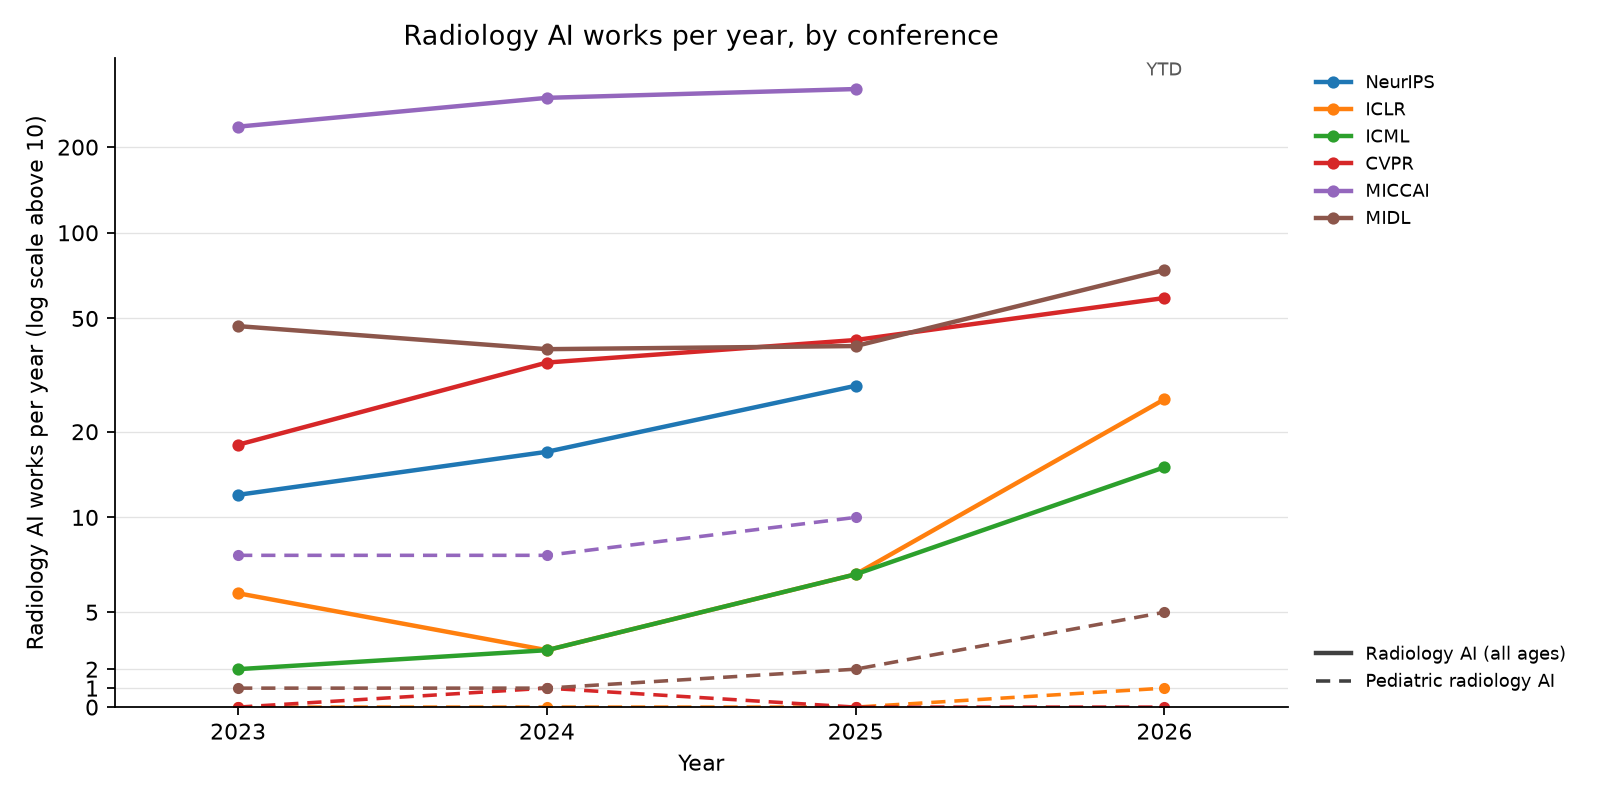
\includegraphics[height=0.82\textheight,width=\textwidth,keepaspectratio]{venue_works_by_year.png}\end{center}
\end{frame}

\begin{frame}[category=Conferences]{NeurIPS: radiology AI works, 2023--2026}
{\scriptsize \textbf{Conference on Neural Information Processing Systems}. Radiology-AI works accepted (from the meeting's paper list), 2023--2026: 58 (2023: 12, 2024: 17, 2025: 29); 0 pediatric (marked $\star$).\par}\vspace{2pt}
\tiny
\begin{adjustbox}{max totalsize={\textwidth}{0.60\textheight}}
\renewcommand{\arraystretch}{1.2}
\begin{tabular}{|l|r|r|>{\raggedright\arraybackslash}p{0.782\textwidth}|}
\hline \textbf{Year} & \textbf{Cites} & \textbf{FWCI} & \textbf{Paper} \\ \hline
2025 & 24 & -- & 3D-RAD: A Comprehensive 3D Radiology Med-VQA Dataset with Multi-Temporal Analysis and Diverse Diagnostic Tasks \\ \hline
2025 & 20 & -- & Better Tokens for Better 3D: Advancing Vision-Language Modeling in 3D Medical Imaging \\ \hline
2024 & 47 & 2.0 & Touchstone Benchmark: Are We on the Right Way for Evaluating AI Algorithms for Medical Segmentation? \\ \hline
2024 & 26 & 0.9 & Eye-gaze Guided Multi-modal Alignment for Medical Representation Learning \\ \hline
2024 & 25 & 1.2 & Enhancing vision-language models for medical imaging: bridging the 3D gap with innovative slice selection \\ \hline
2024 & 20 & -- & DiffusionBlend: Learning 3D Image Prior through Position-aware Diffusion Score Blending for 3D Computed Tomography Reconstruction \\ \hline
2023 & 144 & -- & SegVol: Universal and Interactive Volumetric Medical Image Segmentation \\ \hline
2023 & 104 & -- & LVM-Med: Learning Large-Scale Self-Supervised Vision Models for Medical Imaging via Second-order Graph Matching \\ \hline
2023 & 72 & -- & EHRXQA: A Multi-Modal Question Answering Dataset for Electronic Health Records with Chest X-ray Images \\ \hline
2023 & 66 & -- & SwiFT: Swin 4D fMRI Transformer \\ \hline
2023 & 64 & -- & NeuroGraph: Benchmarks for Graph Machine Learning in Brain Connectomics \\ \hline
2023 & 19 & -- & Knowledge-based in silico models and dataset for the comparative evaluation of mammography AI for a range of breast characteristics, lesion conspicuities and doses \\ \hline
\end{tabular}
\end{adjustbox}
\\[2pt]
\end{frame}

\begin{frame}[category=Conferences]{ICLR: radiology AI works, 2023--2026}
{\scriptsize \textbf{International Conference on Learning Representations}. Radiology-AI works accepted (from the meeting's paper list), 2023--2026: 42 (2023: 6, 2024: 3, 2025: 7, 2026: 26); 1 pediatric (marked $\star$).\par}\vspace{2pt}
\tiny
\begin{adjustbox}{max totalsize={\textwidth}{0.60\textheight}}
\renewcommand{\arraystretch}{1.2}
\begin{tabular}{|l|r|r|>{\raggedright\arraybackslash}p{0.680\textwidth}|}
\hline \textbf{Year} & \textbf{Cites} & \textbf{FWCI} & \textbf{Paper} \\ \hline
2025 & 70 & -- & Large-scale and Fine-grained Vision-language Pre-training for Enhanced CT Image Understanding \\ \hline
2025 & 13 & -- & SimXRD-4M: Big Simulated X-ray Diffraction Data and Crystal Symmetry Classification Benchmark \\ \hline
2025 & 9 & -- & Self-Supervised Diffusion MRI Denoising via Iterative and Stable Refinement \\ \hline
2025 & 9 & -- & Score-based Self-supervised MRI Denoising \\ \hline
2024 & 143 & -- & MMed-RAG: Versatile Multimodal RAG System for Medical Vision Language Models \\ \hline
2024 & 31 & -- & MediConfusion: Can you trust your AI radiologist? Probing the reliability of multimodal medical foundation models \\ \hline
2024 & 19 & -- & The Effect of Intrinsic Dataset Properties on Generalization: Unraveling Learning Differences Between Natural and Medical Images \\ \hline
2024 & 16 & -- & LeFusion: Controllable Pathology Synthesis via Lesion-Focused Diffusion Models \\ \hline
2023 & 107 & -- & Advancing Radiograph Representation Learning with Masked Record Modeling \\ \hline
2023 & 84 & -- & DDM2: Self-Supervised Diffusion MRI Denoising with Generative Diffusion Models \\ \hline
2023 & 40 & -- & AE-FLOW: Autoencoders with Normalizing Flows for Medical Images Anomaly Detection \\ \hline
2023 & 18 & -- & Improved Training of Physics-Informed Neural Networks Using Energy-Based Priors: a Study on Electrical Impedance Tomography \\ \hline
\end{tabular}
\end{adjustbox}
\\[2pt]
\end{frame}

\begin{frame}[category=Conferences]{ICML: radiology AI works, 2023--2026}
{\scriptsize \textbf{International Conference on Machine Learning}. Radiology-AI works accepted (from the meeting's paper list), 2023--2026: 27 (2023: 2, 2024: 3, 2025: 7, 2026: 15); 0 pediatric (marked $\star$).\par}\vspace{2pt}
\tiny
\begin{adjustbox}{max totalsize={\textwidth}{0.60\textheight}}
\renewcommand{\arraystretch}{1.2}
\begin{tabular}{|l|r|r|>{\raggedright\arraybackslash}p{0.748\textwidth}|}
\hline \textbf{Year} & \textbf{Cites} & \textbf{FWCI} & \textbf{Paper} \\ \hline
2025 & 21 & -- & CLIMB: Data Foundations for Large Scale Multimodal Clinical Foundation Models \\ \hline
2025 & 17 & -- & MindLLM: A Subject-Agnostic and Versatile Model for fMRI-to-Text Decoding \\ \hline
2025 & 11 & -- & Raptor: Scalable Train-Free Embeddings for 3D Medical Volumes Leveraging Pretrained 2D Foundation Models \\ \hline
2025 & 5 & -- & Efficient Noise Calculation in Deep Learning-based MRI Reconstructions \\ \hline
2025 & 2 & -- & LangDAug: Langevin Data Augmentation for Multi-Source Domain Generalization in Medical Image Segmentation \\ \hline
2025 & 0 & -- & Staged and Physics-Grounded Learning Framework with Hyperintensity Prior for Pre-Contrast MRI Synthesis \\ \hline
2024 & 14 & -- & Unsupervised Domain Adaptation for Anatomical Structure Detection in Ultrasound Images \\ \hline
2024 & 10 & -- & Adaptive Sampling of k-Space in Magnetic Resonance for Rapid Pathology Prediction \\ \hline
2023 & 17 & -- & ACAT: Adversarial Counterfactual Attention for Classification and Detection in Medical Imaging \\ \hline
2023 & 16 & -- & Robustness of Deep Learning for Accelerated MRI: Benefits of Diverse Training Data \\ \hline
2023 & 15 & -- & Learning High-Order Relationships of Brain Regions \\ \hline
2023 & 8 & -- & Contextualized Policy Recovery: Modeling and Interpreting Medical Decisions with Adaptive Imitation Learning \\ \hline
\end{tabular}
\end{adjustbox}
\\[2pt]
\end{frame}

\begin{frame}[category=Conferences]{CVPR: radiology AI works, 2023--2026}
{\scriptsize \textbf{IEEE/CVF Conference on Computer Vision and Pattern Recognition}. Radiology-AI works accepted (from the meeting's paper list), 2023--2026: 154 (2023: 18, 2024: 35, 2025: 42, 2026: 59); 1 pediatric (marked $\star$).\par}\vspace{2pt}
\tiny
\begin{adjustbox}{max totalsize={\textwidth}{0.60\textheight}}
\renewcommand{\arraystretch}{1.2}
\begin{tabular}{|l|r|r|>{\raggedright\arraybackslash}p{0.680\textwidth}|}
\hline \textbf{Year} & \textbf{Cites} & \textbf{FWCI} & \textbf{Paper} \\ \hline
2025 & 68 & 265.4 & Enhanced Contrastive Learning with Multi-view Longitudinal Data for Chest X-ray Report Generation \\ \hline
2024 & 84 & 47.9 & Towards Generalizable Tumor Synthesis \\ \hline
2024 & 81 & 14.6 & Rethinking Diffusion Model for Multi-Contrast MRI Super-Resolution \\ \hline
2024 & 73 & 13.8 & MemSAM: Taming Segment Anything Model for Echocardiography Video Segmentation \\ \hline
2023 & 243 & 20.2 & Dynamic Graph Enhanced Contrastive Learning for Chest X-Ray Report Generation \\ \hline
2023 & 222 & 75.5 & Ambiguous Medical Image Segmentation Using Diffusion Models \\ \hline
2023 & 217 & 18.7 & METransformer: Radiology Report Generation by Transformer with Multiple Learnable Expert Tokens \\ \hline
2023 & 164 & 21.9 & MCF: Mutual Correction Framework for Semi-Supervised Medical Image Segmentation \\ \hline
2023 & 133 & 14.4 & KiUT: Knowledge-injected U-Transformer for Radiology Report Generation \\ \hline
2023 & 117 & 67.2 & Structure-Aware Sparse-View X-Ray 3D Reconstruction \\ \hline
2023 & 103 & 11.0 & Label-Free Liver Tumor Segmentation \\ \hline
2023 & 75 & 14.1 & Learning Federated Visual Prompt in Null Space for MRI Reconstruction \\ \hline
\end{tabular}
\end{adjustbox}
\\[2pt]
\end{frame}

\begin{frame}[category=Conferences]{MICCAI: radiology AI works, 2023--2026}
{\scriptsize \textbf{Medical Image Computing and Computer-Assisted Intervention}. Radiology-AI works accepted (from the meeting's paper list), 2023--2026: 854 (2023: 236, 2024: 298, 2025: 320); 26 pediatric (marked $\star$).\par}\vspace{2pt}
\tiny
\begin{adjustbox}{max totalsize={\textwidth}{0.60\textheight}}
\renewcommand{\arraystretch}{1.2}
\begin{tabular}{|l|r|r|>{\raggedright\arraybackslash}p{0.680\textwidth}|}
\hline \textbf{Year} & \textbf{Cites} & \textbf{FWCI} & \textbf{Paper} \\ \hline
2025 & 208 & 1.1 & MedVLM-R1: Incentivizing Medical Reasoning Capability of Vision-Language Models (VLMs) via Reinforcement Learning \\ \hline
2024 & 133 & -- & CT2Rep: Automated Radiology Report Generation for 3D Medical Imaging \\ \hline
2024 & 102 & -- & Anatomically-Controllable Medical Image Generation with Segmentation-Guided Diffusion Models \\ \hline
2024 & 87 & -- & MedCLIP-SAM: Bridging Text and Image Towards Universal Medical Image Segmentation \\ \hline
2023 & 462 & -- & MedNeXt: Transformer-driven Scaling of ConvNets for Medical Image Segmentation \\ \hline
2023 & 128 & -- & CoLa-Diff: Conditional Latent Diffusion Model for Multi-Modal MRI Synthesis \\ \hline
2023 & 105 & -- & DiffMIC: Dual-Guidance Diffusion Network for Medical Image Classification \\ \hline
2023 & 97 & 13.9 & Beyond Adapting SAM: Towards End-to-End Ultrasound Image Segmentation via Auto Prompting \\ \hline
2023 & 95 & -- & Self-Supervised MRI Reconstruction with Unrolled Diffusion Models \\ \hline
2023 & 83 & -- & Make-A-Volume: Leveraging Latent Diffusion Models for Cross-Modality 3D Brain MRI Synthesis \\ \hline
2023 & 72 & 19.0 & BerDiff: Conditional Bernoulli Diffusion Model for Medical Image Segmentation \\ \hline
2023 & 71 & -- & Ariadne's Thread: Using Text Prompts to Improve Segmentation of Infected Areas from Chest X-ray images \\ \hline
\end{tabular}
\end{adjustbox}
\\[2pt]
\end{frame}

\begin{frame}[category=Conferences]{MIDL: radiology AI works, 2023--2026}
{\scriptsize \textbf{Medical Imaging with Deep Learning}. Radiology-AI works accepted (from the meeting's paper list), 2023--2026: 200 (2023: 47, 2024: 39, 2025: 40, 2026: 74); 9 pediatric (marked $\star$).\par}\vspace{2pt}
\tiny
\begin{adjustbox}{max totalsize={\textwidth}{0.60\textheight}}
\renewcommand{\arraystretch}{1.2}
\begin{tabular}{|l|r|r|>{\raggedright\arraybackslash}p{0.680\textwidth}|}
\hline \textbf{Year} & \textbf{Cites} & \textbf{FWCI} & \textbf{Paper} \\ \hline
2024 & 14 & -- & Imbalance-aware loss functions improve medical image classification \\ \hline
2023 & 78 & -- & Patched Diffusion Models for Unsupervised Anomaly Detection in Brain MRI \\ \hline
2023 & 39 & -- & MMCFormer: Missing Modality Compensation Transformer for Brain Tumor Segmentation \\ \hline
2023 & 29 & -- & Medical diffusion on a budget: textual inversion for medical image generation \\ \hline
2023 & 23 & -- & MProtoNet: A Case-Based Interpretable Model for Brain Tumor Classification with 3D Multi-parametric Magnetic Resonance Imaging \\ \hline
2023 & 22 & -- & Diffusion Models for Contrast Harmonization of Magnetic Resonance Images \\ \hline
2023 & 20 & -- & Exploring Image Augmentations for Siamese Representation Learning with Chest X-Rays \\ \hline
2023 & 19 & -- & 3D Medical Axial Transformer: A Lightweight Transformer Model for 3D Brain Tumor Segmentation \\ \hline
2023 & 19 & -- & Vision-Language Modelling For Radiological Imaging and Reports In The Low Data Regime \\ \hline
2023 & 14 & -- & E(3) x SO(3)-Equivariant Networks for Spherical Deconvolution in Diffusion MRI \\ \hline
2023 & 14 & -- & Amortized Normalizing Flows for Transcranial Ultrasound with Uncertainty Quantification \\ \hline
2023 & 13 & -- & Selective experience replay compression using coresets for lifelong deep reinforcement learning in medical imaging \\ \hline
\end{tabular}
\end{adjustbox}
\\[2pt]
\end{frame}

\begin{frame}[category=Conferences]{MICCAI: pediatric radiology AI works (1/2)}
\relax{\scriptsize 26 pediatric radiology-AI papers accepted 2023--2026 (21 fetal, 4 infant / neonatal, 1 pediatric). Meetings with a published paper list: 2023, 2024, 2025.\par}\vspace{2pt}
\tiny
\begin{adjustbox}{max totalsize={\textwidth}{0.66\textheight}}
\renewcommand{\arraystretch}{1.2}
\begin{tabular}{|l|l|>{\raggedright\arraybackslash}p{0.792\textwidth}|}
\hline \textbf{Year} & \textbf{Population} & \textbf{Paper} \\ \hline
2025 & Fetal & Accurate and Efficient Fetal Birth Weight Estimation from 3D Ultrasound \\ \hline
2025 & Fetal & Adaptive Frame Selection for Gestational Age Estimation from Blind Sweep Fetal Ultrasound Videos \\ \hline
2025 & Infant / neonatal & Flexibly Distilled 3D Rectified Flow with Anatomical Constraints for Developmental Infant Brain MRI Prediction \\ \hline
2025 & Fetal & Fusing Radiomic Features with Deep Representations for Gestational Age Estimation in Fetal Ultrasound Images \\ \hline
2025 & Fetal & General Methods Make Great Domain-specific Foundation Models: A Case-study on Fetal Ultrasound \\ \hline
2025 & Fetal & Influence of Classification Task and Distribution Shift Type on OOD Detection in Fetal Ultrasound \\ \hline
2025 & Fetal & Latent Motion Profiling for Annotation-free Cardiac Phase Detection in Adult and Fetal Echocardiography Videos \\ \hline
2025 & Fetal & Robust Fetal Pose Estimation across Gestational Ages via Cross-Population Augmentation \\ \hline
2025 & Fetal & Self-supervised Normality Learning and Divergence Vector-guided Model Merging for Zero-shot Congenital Heart Disease Detection in Fetal Ultrasound Videos \\ \hline
2025 & Fetal & You Can Detect It: Fetal Biometric Estimation Using Ellipse Detection \\ \hline
2024 & Fetal & Cycle-consistent Learning for Fetal Cortical Surface Reconstruction \\ \hline
2024 & Pediatric & Efficient and Gender-adaptive Graph Vision Mamba for Pediatric Bone Age Assessment \\ \hline
2024 & Fetal & Fetal MRI Reconstruction by Global Diffusion and Consistent Implicit Representation \\ \hline
2024 & Fetal & Geometric Transformation Uncertainty for Improving 3D Fetal Brain Pose Prediction from Freehand 2D Ultrasound Videos \\ \hline
\end{tabular}
\end{adjustbox}
\\[2pt]
{\tiny Source: the meeting's accepted-paper list; a title counts when it names an imaging modality, an AI method and a pediatric term (fetal included). Titles only, so pediatric work that does not say so in its title is missed.}
\end{frame}

\begin{frame}[category=Conferences]{MICCAI: pediatric radiology AI works (2/2)}
\relax{\scriptsize 26 pediatric radiology-AI papers accepted 2023--2026 (21 fetal, 4 infant / neonatal, 1 pediatric). Meetings with a published paper list: 2023, 2024, 2025.\par}\vspace{2pt}
\tiny
\begin{adjustbox}{max totalsize={\textwidth}{0.66\textheight}}
\renewcommand{\arraystretch}{1.2}
\begin{tabular}{|l|l|>{\raggedright\arraybackslash}p{0.720\textwidth}|}
\hline \textbf{Year} & \textbf{Population} & \textbf{Paper} \\ \hline
2024 & Fetal & Improving cross-domain brain tissue segmentation in fetal MRI with synthetic data \\ \hline
2024 & Fetal & Intrapartum Ultrasound Image Segmentation of Pubic Symphysis and Fetal Head Using Dual Student-Teacher Framework with CNN-ViT Collaborative Learning \\ \hline
2024 & Fetal & Pose-GuideNet: Automatic Scanning Guidance for Fetal Head Ultrasound from Pose Estimation \\ \hline
2024 & Infant / neonatal & Super-Field MRI Synthesis for Infant Brains Enhanced by Dual Channel Latent Diffusion \\ \hline
2023 & Fetal & An automated pipeline for quantitative T2* fetal body MRI and segmentation at low field \\ \hline
2023 & Fetal & ASC: Appearance and Structure Consistency for Unsupervised Domain Adaptation in Fetal Brain MRI Segmentation \\ \hline
2023 & Fetal & Dual Conditioned Diffusion Models for Out-Of-Distribution Detection: Application to Fetal Ultrasound Videos \\ \hline
2023 & Fetal & Improving Automatic Fetal Biometry Measurement with Swoosh Activation Function \\ \hline
2023 & Infant / neonatal & Punctate White Matter Lesion Segmentation in Preterm Infants Powered by Counterfactually Generative Learning \\ \hline
2023 & Fetal & Simulation-based parameter optimization for fetal brain MRI super-resolution reconstruction \\ \hline
2023 & Infant / neonatal & SurfFlow: A Flow-Based Approach for Rapid and Accurate Cortical Surface Reconstruction from Infant Brain MRI \\ \hline
2023 & Fetal & UM-CAM: Uncertainty-weighted Multi-resolution Class Activation Maps for Weakly-supervised Fetal Brain Segmentation \\ \hline
\end{tabular}
\end{adjustbox}
\\[2pt]
{\tiny Source: the meeting's accepted-paper list; a title counts when it names an imaging modality, an AI method and a pediatric term (fetal included). Titles only, so pediatric work that does not say so in its title is missed.}
\end{frame}

\begin{frame}[category=Conferences]{MIDL: pediatric radiology AI works}
\relax{\scriptsize 9 pediatric radiology-AI papers accepted 2023--2026 (7 fetal, 2 pediatric). Meetings with a published paper list: 2023, 2024, 2025, 2026.\par}\vspace{2pt}
\tiny
\begin{adjustbox}{max totalsize={\textwidth}{0.66\textheight}}
\renewcommand{\arraystretch}{1.2}
\begin{tabular}{|l|l|>{\raggedright\arraybackslash}p{0.720\textwidth}|}
\hline \textbf{Year} & \textbf{Population} & \textbf{Paper} \\ \hline
2026 & Fetal & Calibration-Aware Semi-Supervised Fetal Head Segmentation with Boundary-Positive Contrast \\ \hline
2026 & Fetal & Orientation-Aware Diffusion Super-Resolution for 3T-Like Fetal MRI from Routine 1.5T Scans \\ \hline
2026 & Fetal & SuD-CoTAN: Sulcal Depth-guided Anatomically Consistent Fetal Cortical Surface Reconstruction \\ \hline
2026 & Fetal & Ultra-ECP: Ellipse-Constrained and Point-Robust Foundation Model Adaptation for Fetal Cardiac Ultrasound Segmentation \\ \hline
2026 & Pediatric & WristMIR: Coarse-to-Fine Region-Aware Retrieval of Pediatric Wrist Radiographs with Radiology Report-Driven Learning \\ \hline
2025 & Fetal & FERN: A Fetal Echocardiography Registration Network for 2D-to-3D Alignment \\ \hline
2025 & Pediatric & GAMBAS: Generalised-Hilbert Mamba for Super-resolution of Paediatric Ultra-Low-Field MRI \\ \hline
2024 & Fetal & Joint Motion Estimation with Geometric Deformation Correction for Fetal Echo Planar Images Via Deep Learning \\ \hline
2023 & Fetal & FUSQA: Fetal Ultrasound Segmentation Quality Assessment \\ \hline
\end{tabular}
\end{adjustbox}
\\[2pt]
{\tiny Source: the meeting's accepted-paper list; a title counts when it names an imaging modality, an AI method and a pediatric term (fetal included). Titles only, so pediatric work that does not say so in its title is missed.}
\end{frame}

\begin{frame}[category=Journals]{AI fracture detection in a real pediatric emergency department}
{\scriptsize Ziegner et al., European Radiology 2025 (second most-cited pediatric paper of 2025)\par}\vspace{2pt}
\begin{columns}[T]
\begin{column}{0.42\textwidth}\centering
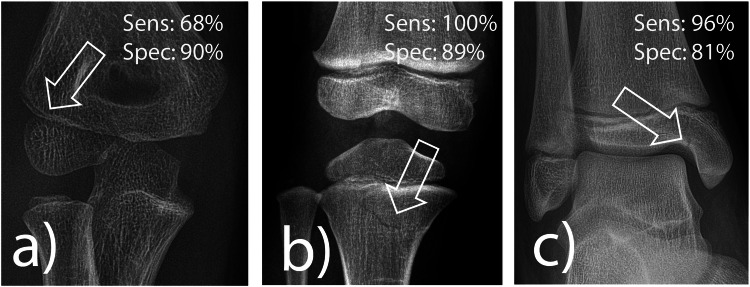
\includegraphics[height=0.50\textheight,width=\textwidth,keepaspectratio]{examples/spot_fracture_ed.jpg}\\[2pt]
{\tiny Ziegner et al., Eur Radiol 2025, figure 4: pediatric fractures the software found, with its per-region sensitivity and specificity}\\{\tiny source: cdn.ncbi.nlm.nih.gov}
\end{column}
\begin{column}{0.56\textwidth}
\scriptsize\setlength{\itemsep}{1pt}
\begin{itemize}
\item \textbf{Problem}: fractures in children are missed most often by the least experienced readers, at night, in the emergency department.
\item \textbf{Data}: 1,672 consecutive radiographs of children under 18 from one tertiary pediatric emergency department, plus a selected medicolegal set (proximal tibia, radial condyle); three pediatric residents read each before and after seeing the AI.
\item \textbf{Method}: a commercially available, CE-marked deep-learning fracture detector (adult-derived, pediatric extension) run stand-alone and as a second reader.
\item \textbf{Result}: stand-alone sensitivity 92\%, specificity 83\%; 100\% for proximal tibia but 68\% for radial condyle fractures; residents' accuracy rose from 88\% to 90\%, and in 2\% of cases they dropped a correct diagnosis after seeing the AI.
\item \textbf{Why it matters}: the first real-life pediatric ED evaluation: the gain from a cleared adult tool is real but modest, and the elbow remains the weak spot.
\end{itemize}
\end{column}
\end{columns}
\end{frame}

\begin{frame}[category=Journals]{pTBLightNet: pediatric tuberculosis on frontal and lateral chest radiographs}
{\scriptsize Capellán-Martín et al., Nature Communications 2025 (open access)\par}\vspace{2pt}
\begin{columns}[T]
\begin{column}{0.42\textwidth}\centering
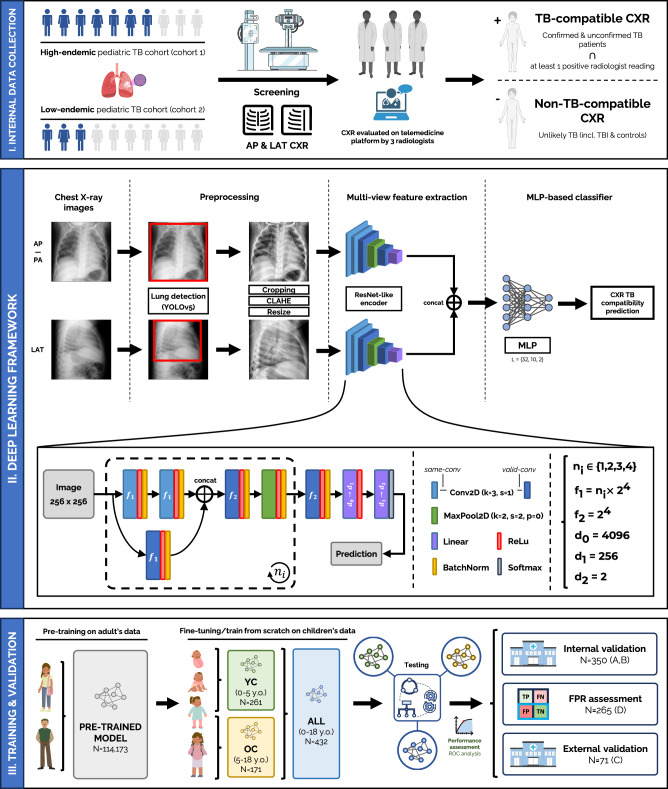
\includegraphics[height=0.50\textheight,width=\textwidth,keepaspectratio]{examples/spot_ped_tb.jpg}\\[2pt]
{\tiny Capellan-Martin et al., Nat Commun 2025, figure 1: the multi-view pTBLightNet pipeline}\\{\tiny source: cdn.ncbi.nlm.nih.gov}
\end{column}
\begin{column}{0.56\textwidth}
\scriptsize\setlength{\itemsep}{1pt}
\begin{itemize}
\item \textbf{Problem}: pediatric pulmonary TB has vaguer symptoms and subtler radiographs than adult TB; most affected children in high-burden settings are never diagnosed.
\item \textbf{Data}: pre-trained on 114,173 adult chest radiographs, then fine-tuned and tested on 918 radiographs from three pediatric TB cohorts, with lateral views.
\item \textbf{Method}: a multi-view network that scores frontal and lateral films for TB-compatible findings; separate models for under-5 and 5-18 years.
\item \textbf{Result}: AUC 0.90 on internal and 0.68 on external testing; lateral views helped most in the youngest children; age-specific models matched larger undifferentiated ones.
\item \textbf{Why it matters}: shows both the value of adult pre-training for a rare pediatric target and the internal-to-external drop that every pediatric deployment should expect.
\end{itemize}
\end{column}
\end{columns}
\end{frame}

\begin{frame}[category=Journals]{Deep-learning reconstruction shortens pediatric brain MRI}
{\scriptsize Yoo et al., Korean Journal of Radiology 2025 (open access)\par}\vspace{2pt}
\begin{columns}[T]
\begin{column}{0.42\textwidth}\centering
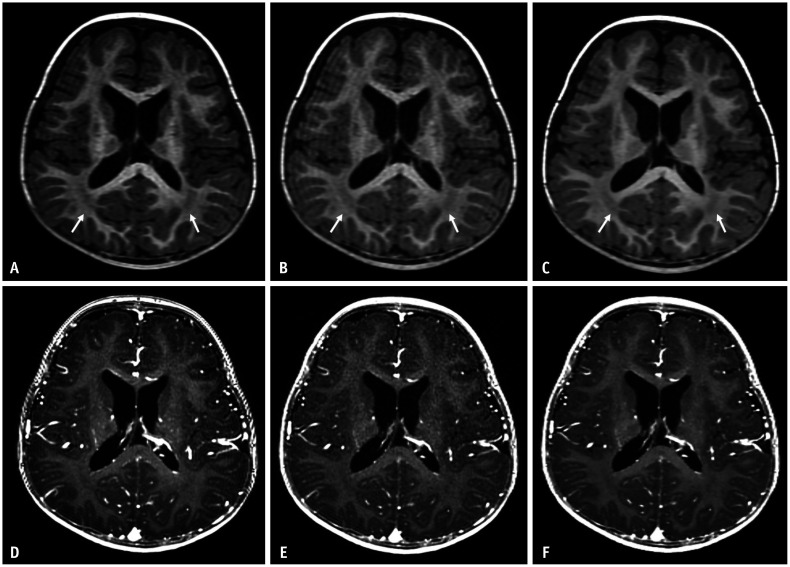
\includegraphics[height=0.50\textheight,width=\textwidth,keepaspectratio]{examples/spot_dl_recon_mri.jpg}\\[2pt]
{\tiny Yoo et al., Korean J Radiol 2025, figure 2: conventional (A, D) vs accelerated 3D T1 pediatric brain MRI without (B, E) and with (C, F) deep-learning reconstruction}\\{\tiny source: cdn.ncbi.nlm.nih.gov}
\end{column}
\begin{column}{0.56\textwidth}
\scriptsize\setlength{\itemsep}{1pt}
\begin{itemize}
\item \textbf{Problem}: long 3D T1 sequences are where children move, sedation is prescribed, and scanner time is lost.
\item \textbf{Data}: 46 children scanned with both the conventional and an accelerated 3D T1 protocol (pre- and post-contrast) on one 3T scanner.
\item \textbf{Method}: vendor deep-learning reconstruction applied to the accelerated acquisition; noise, contrast, signal-to-noise and radiologist ratings compared with the conventional scan.
\item \textbf{Result}: acquisition time cut by 29\% (pre-contrast) and 41\% (post-contrast); the deep-learning images had lower noise, higher SNR and CNR, better overall quality and fewer artifacts than the conventional scan.
\item \textbf{Why it matters}: reconstruction AI is on the scanner today and gives children a shorter, better exam without any diagnostic model in the loop.
\end{itemize}
\end{column}
\end{columns}
\end{frame}

\begin{frame}[category=Journals]{Deeplasia bone age in rare growth disorders, against multiple experts}
{\scriptsize Skaf et al., Frontiers in Endocrinology 2026 (open access); external validation of Rassmann et al., Pediatr Radiol 2023\par}\vspace{2pt}
\begin{columns}[T]
\begin{column}{0.42\textwidth}\centering
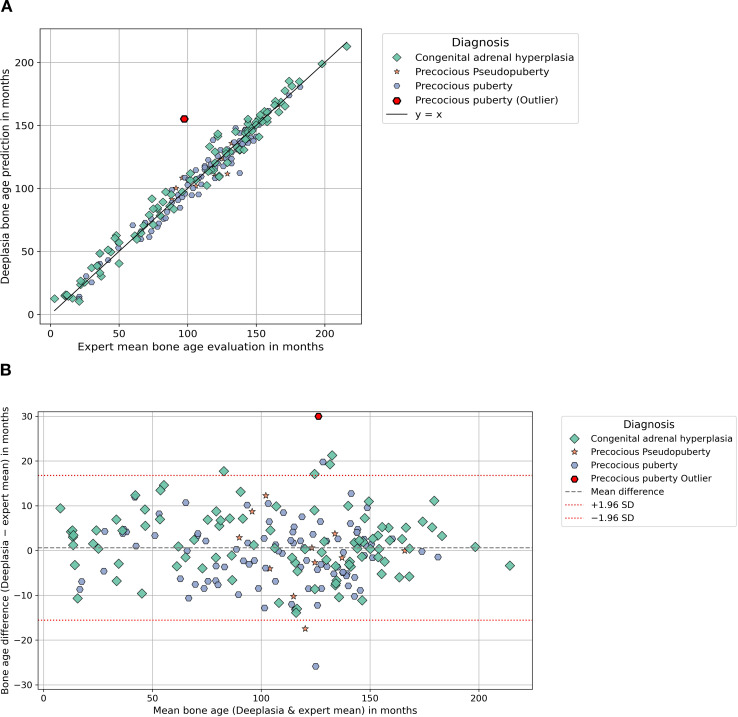
\includegraphics[height=0.50\textheight,width=\textwidth,keepaspectratio]{examples/spot_deeplasia_rare.jpg}\\[2pt]
{\tiny Skaf et al., Front Endocrinol 2026, figure 1: Deeplasia bone age vs the expert mean in the endocrine cohort (scatter and Bland-Altman)}\\{\tiny source: cdn.ncbi.nlm.nih.gov}
\end{column}
\begin{column}{0.56\textwidth}
\scriptsize\setlength{\itemsep}{1pt}
\begin{itemize}
\item \textbf{Problem}: bone-age models are trained on ordinary hands; the children who need bone age most have syndromes, endocrine disease or lysosomal storage disorders that distort the skeleton.
\item \textbf{Data}: 1,138 hand radiographs from several centers: SHOX deficiency, Noonan, Silver-Russell, Turner, CAH, precocious puberty (cohort 1) and mucopolysaccharidoses and other storage disorders (cohort 2); two to five expert Greulich-Pyle readings each.
\item \textbf{Method}: the open-source Deeplasia system run unchanged; each human rater and the model scored against the remaining experts.
\item \textbf{Result}: mean absolute error 6.0 months (cohort 1) and 7.1 months (storage disorders), 1-year accuracy 90\% and 81\%; the model beat every individual human rater.
\item \textbf{Why it matters}: an open pediatric model validated on the hardest cases, by an outside group, on external data: the template for how a children's hospital should test any tool.
\end{itemize}
\end{column}
\end{columns}
\end{frame}

\begin{frame}[category=Journals]{Pediatric PET at one fifth of the counts with patch-based deep learning}
{\scriptsize Han et al., EJNMMI Physics 2026 (open access; Cincinnati Children's)\par}\vspace{2pt}
\begin{columns}[T]
\begin{column}{0.42\textwidth}\centering
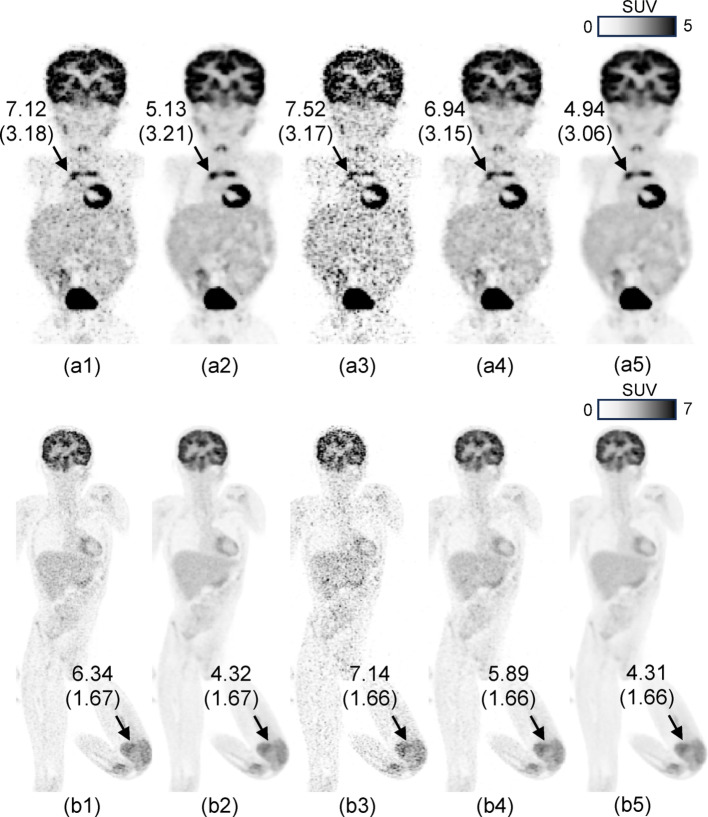
\includegraphics[height=0.50\textheight,width=\textwidth,keepaspectratio]{examples/spot_pet_dose.jpg}\\[2pt]
{\tiny Han et al., EJNMMI Phys 2026, figure 5: pediatric whole-body FDG PET, standard 90 s vs 20 s per bed, with and without patch-based deep-learning denoising}\\{\tiny source: cdn.ncbi.nlm.nih.gov}
\end{column}
\begin{column}{0.56\textwidth}
\scriptsize\setlength{\itemsep}{1pt}
\begin{itemize}
\item \textbf{Problem}: PET dose and scan time in children are set by noise; conventional denoising networks need large training sets that pediatric PET does not have.
\item \textbf{Data}: one high-quality pediatric exam for training; a NEMA phantom and 88 clinical whole-body FDG exams (under 12 years) with list-mode data truncated from 90 s to 20 s per bed.
\item \textbf{Method}: a patch-based network that learns local structure from a single exam and denoises the reduced-count images; blinded observer study and SUV analysis.
\item \textbf{Result}: 20-second images rated equal or better than the standard 90-second images in more than 85\% of cases, with resolution, contrast and SUV preserved.
\item \textbf{Why it matters}: either a 4.5x shorter scan or about 22\% of today's injected activity, from a method trainable on a single local exam.
\end{itemize}
\end{column}
\end{columns}
\end{frame}

\begin{frame}[category=Journals]{Children are not small adults: an adult CT segmentation model in children}
{\scriptsize Chatterjee et al., Journal of Imaging Informatics in Medicine 2025\par}\vspace{2pt}
\begin{columns}[T]
\begin{column}{0.42\textwidth}\centering
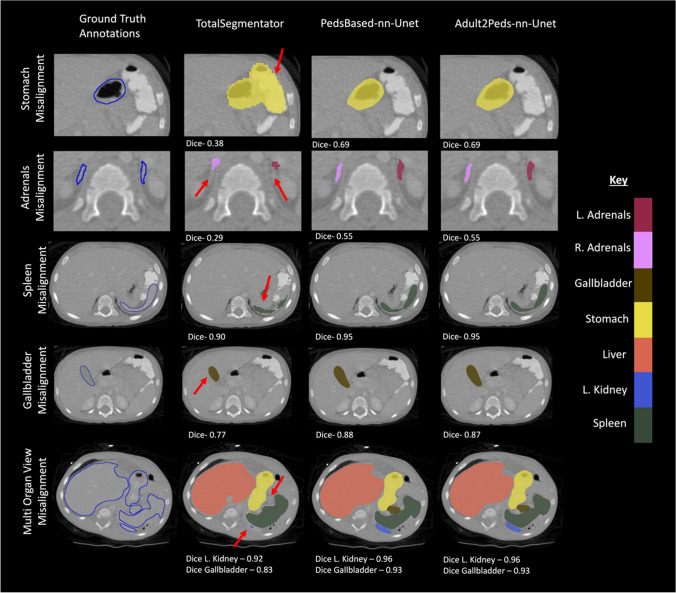
\includegraphics[height=0.50\textheight,width=\textwidth,keepaspectratio]{examples/spot_not_small_adults.jpg}\\[2pt]
{\tiny Chatterjee et al., J Imaging Inform Med 2025, figure 7: pediatric CT organ labels, ground truth vs adult-trained TotalSegmentator vs pediatric-trained models}\\{\tiny source: cdn.ncbi.nlm.nih.gov}
\end{column}
\begin{column}{0.56\textwidth}
\scriptsize\setlength{\itemsep}{1pt}
\begin{itemize}
\item \textbf{Problem}: the most-used open CT organ segmentation model (TotalSegmentator) was trained on adults; nobody had measured how it behaves in children.
\item \textbf{Data}: external adult (n = 300) and pediatric (n = 359) abdominal CT sets with expert organ labels.
\item \textbf{Method}: TotalSegmentator scored on both sets; then a pediatric-only nnU-Net and an adult model fine-tuned on pediatric cases.
\item \textbf{Result}: mean Dice fell from 0.81 in adults to 0.73 in children, worst for the adrenals (0.69 to 0.41 and 0.35), duodenum and pancreas; pediatric training or fine-tuning recovered the loss.
\item \textbf{Why it matters}: the clearest quantitative case for local pediatric validation and fine-tuning of adult-derived tools before clinical use.
\end{itemize}
\end{column}
\end{columns}
\end{frame}


\begin{frame}[category=Datasets]{The biggest public pediatric radiology AI datasets}
\tiny
\begin{adjustbox}{max totalsize={\textwidth}{0.70\textheight}}
\renewcommand{\arraystretch}{1.2}
\begin{tabular}{|>{\raggedright\arraybackslash}p{0.284\textwidth}|l|>{\raggedright\arraybackslash}p{0.189\textwidth}|>{\raggedright\arraybackslash}p{0.284\textwidth}|>{\raggedright\arraybackslash}p{0.095\textwidth}|>{\raggedright\arraybackslash}p{0.135\textwidth}|}
\hline \textbf{Dataset} & \textbf{Year} & \textbf{Modality} & \textbf{Size} & \textbf{Ages} & \textbf{Access} \\ \hline
CBTN clinical MRI (Children's Brain Tumor Network) & 2023 & brain / spine tumor MRI & 23,101 exams (1,526 patients); tumor masks for 370 & pediatric & application (NCI CCDI) \\ \hline
GRAZPEDWRI-DX & 2022 & wrist radiographs (trauma) & 20,327 images (6,091 patients) & 0.2--19 y & open \\ \hline
RSNA Pediatric Bone Age Challenge & 2017 & hand radiographs & 14,236 images (bone age + sex) & mean 10.6 y & open (RSNA terms) \\ \hline
FETAL\_PLANES\_DB & 2020 & fetal ultrasound (standard planes) & 12,400 images (1,792 pregnancies) & fetal & open \\ \hline
ABCD Study & 2018-- & brain MRI, longitudinal & 11,878 participants, up to 7 follow-ups & 9--10 y at baseline & application (NBDC) \\ \hline
PediCXR / VinDr-PCXR & 2023 & chest radiographs & 9,125 studies; 36 findings, 15 diagnoses & \textless{} 10 y & credentialed (PhysioNet) \\ \hline
Guangzhou pediatric chest X-ray (Kermany) & 2018 & chest radiographs & 5,856 images (normal / bacterial / viral pneumonia) & 1--5 y & open \\ \hline
ABIDE I + II (autism) & 2012 / 2016 & brain MRI (structural, resting fMRI) & 2,156 subjects & 5--64 y (mostly children) & open \\ \hline
Regensburg Pediatric Appendicitis & 2023 & abdominal ultrasound + labs & 1,709 images (579 patients) & 0--18 y & open \\ \hline
dHCP (Developing Human Connectome Project) & 2022--24 & neonatal + fetal brain MRI & 886 neonatal + 297 fetal datasets, with segmentations & 20--45 weeks & open (NDA) \\ \hline
Pediatric-CT-SEG (TCIA) & 2022 & chest / abdomen / pelvis CT & 718 series (359 patients); 29 organ contours & 5 days -- 16 y & open \\ \hline
BraTS-PEDs (pediatric brain tumor challenge) & 2023--25 & brain tumor MRI & 464 patients (2024 challenge); 1,649 series on TCIA & pediatric & registration / TCIA \\ \hline
FeTA (fetal brain tissue annotation) & 2021--24 & fetal brain MRI & 280 volumes (120 train + 160 test); 7 tissue labels & 18--35 weeks & registration \\ \hline
\end{tabular}
\end{adjustbox}
\\[3pt]
{\tiny Sizes verified against the primary paper or hosting page (2026-09). Only two pediatric radiograph sets exceed
10,000 images; the largest public pediatric-only CT set has 359 patients; no RSNA pediatric challenge has run since
bone age in 2017. Adult benchmarks (CheXpert 224k, MIMIC-CXR 377k) exclude children.}
\end{frame}

\begin{frame}[category=Newsletters]{Radiology AI newsletter stories per year, by source}
\begin{center}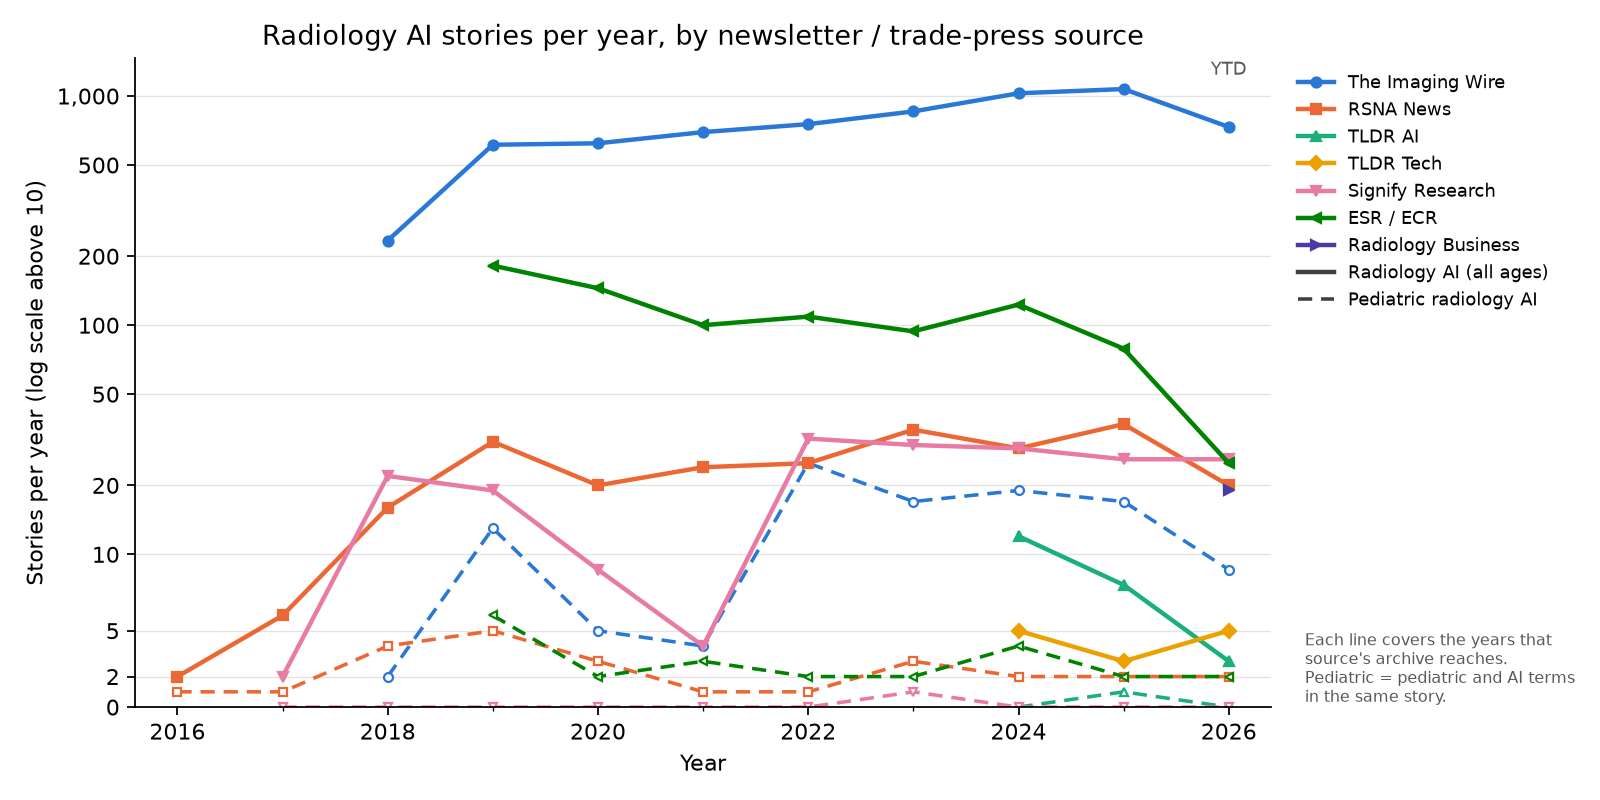
\includegraphics[height=0.82\textheight,width=\textwidth,keepaspectratio]{newsletter_by_source.png}\end{center}
\end{frame}

\begin{frame}[category=Newsletters]{Pediatric radiology AI in the trade press, 2023 (23 stories)}
\tiny
\begin{adjustbox}{max totalsize={\textwidth}{0.84\textheight}}
\renewcommand{\arraystretch}{1.2}
\begin{tabular}{|l|l|>{\raggedright\arraybackslash}p{0.581\textwidth}|>{\raggedright\arraybackslash}p{0.270\textwidth}|}
\hline \textbf{Date} & \textbf{Newsletter} & \textbf{Story} & \textbf{Paper} \\ \hline
2023-01-08 & The Imaging Wire & Gestational Age AI &  \\ \hline
2023-03-01 & The Imaging Wire & Fetal Ultrasound AI Generalizability & Sendra-Balcells et al., 2023 (Scientific Reports) \\ \hline
2023-03-08 & ESR / ECR & ECR 2023 -- A true celebration of the cycle of life. &  \\ \hline
2023-03-17 & The Imaging Wire & When Sao Paolo's Diagnosticos da America (DASA, the world's fourth largest diagn &  \\ \hline
2023-04-07 & The Imaging Wire & Ultrasound Spots Breech Pregnancies & Knights et al., 2023 (PLOS Medicine) \\ \hline
2023-04-07 & The Imaging Wire & When Sao Paolo's Diagnosticos da America SA (DASA, the world's fourth largest di &  \\ \hline
2023-04-12 & Signify Research & Where do opportunities exist? &  \\ \hline
2023-04-12 & RSNA News & RSNA Webinar to Examine Impact of Large Language Models &  \\ \hline
2023-05-07 & The Imaging Wire & New C-Arm Launched &  \\ \hline
2023-06-07 & The Imaging Wire & BrightHeart's Fetal Heart AI &  \\ \hline
2023-06-12 & RSNA News & Understanding the Imaging Spectrum of non-Hodgkin Lymphoma in Children, Adolescents and Young Adults &  \\ \hline
2023-06-19 & The Imaging Wire & Better Together at SIIM &  \\ \hline
2023-06-25 & The Imaging Wire & AI Detects Child Abuse on CT &  \\ \hline
2023-07-07 & RSNA News & Survivors of Childhood Cancer: Risk of Future Disease, Screening Needs and the Role of Radiology &  \\ \hline
2023-08-02 & The Imaging Wire & MRI Radiomics Hones in on Crohn's & Liu et al., 2024 (American Journal of Roentgenology) \\ \hline
2023-08-02 & The Imaging Wire & Sonio Gets FDA Nod for Fetal AI &  \\ \hline
2023-09-20 & The Imaging Wire & GE Lands \$44M AI Ultrasound Grant &  \\ \hline
2023-10-08 & The Imaging Wire & ChatGPT Reports for Patients & Jeblick et al., 2023 (European Radiology) \\ \hline
2023-11-08 & The Imaging Wire & Philips to Expand AI-Powered POCUS &  \\ \hline
2023-11-08 & The Imaging Wire & Stories of Success in Cloud and AI &  \\ \hline
2023-11-12 & The Imaging Wire & Uneven Success Against Breast Cancer | Pediatric Radiation &  \\ \hline
2023-11-26 & The Imaging Wire & AI of MRI Diagnoses Autism &  \\ \hline
2023-12-11 & ESR / ECR & Revolutionising paediatric radiology: the future impact of AI &  \\ \hline
\end{tabular}
\end{adjustbox}
\end{frame}

\begin{frame}[category=Newsletters]{Pediatric radiology AI in the trade press, 2024 (25 stories)}
\tiny
\begin{adjustbox}{max totalsize={\textwidth}{0.84\textheight}}
\renewcommand{\arraystretch}{1.2}
\begin{tabular}{|l|l|>{\raggedright\arraybackslash}p{0.559\textwidth}|>{\raggedright\arraybackslash}p{0.260\textwidth}|}
\hline \textbf{Date} & \textbf{Newsletter} & \textbf{Story} & \textbf{Paper} \\ \hline
2024-01-10 & The Imaging Wire & AI Models Go Head-to-Head in Project AIR Study & van Leeuwen et al., 2024 (Radiology) \\ \hline
2024-01-15 & ESR / ECR & Hidden health risks of endocrine disruptors? &  \\ \hline
2024-01-17 & The Imaging Wire & Echo AI's RHD Impact & Brown et al., 2024 (Journal of the American Heart Association) \\ \hline
2024-01-20 & The Imaging Wire & Us2.ai &  \\ \hline
2024-02-07 & The Imaging Wire & Meet Gleamer at ECR 2024 &  \\ \hline
2024-03-20 & The Imaging Wire & AI Helps Residents Detect Fractures &  \\ \hline
2024-04-22 & The Imaging Wire & GE Launches US Scanners &  \\ \hline
2024-05-19 & The Imaging Wire & Early Preeclampsia Risk Screening & Guerby et al., 2024 (Hypertension) \\ \hline
2024-06-29 & The Imaging Wire & FDA Clears New Clarius Prenatal App &  \\ \hline
2024-07-01 & ESR / ECR & AI applications in musculoskeletal imaging &  \\ \hline
2024-07-10 & RSNA News & Experts Outline Considerations to Deploy AI in Radiology &  \\ \hline
2024-08-14 & The Imaging Wire & Cardiac Ultrasound Scanner Cleared &  \\ \hline
2024-08-25 & The Imaging Wire & When Follow-Up Falls Short | Pediatric CT Use &  \\ \hline
2024-08-25 & The Imaging Wire & MAUI Emerges from Stealth &  \\ \hline
2024-09-04 & The Imaging Wire & Samsung Finalizes Sonio Acquisition &  \\ \hline
2024-09-08 & The Imaging Wire & AZmed AI Extended to Kids &  \\ \hline
2024-10-03 & ESR / ECR & On Artificial Intelligence: An interview with Susan Shelmerdine &  \\ \hline
2024-10-06 & The Imaging Wire & Fracture AI Improves Over Time &  \\ \hline
2024-10-10 & The Imaging Wire & Low-Dose CT in Kids | Hinton Nabs Nobel, Cancels MRI &  \\ \hline
2024-10-10 & The Imaging Wire & Low-Dose CT Confounds CAD in Kids & Hardie et al., 2025 (American Journal of Roentgenology) \\ \hline
2024-10-17 & ESR / ECR & On Artificial Intelligence: An interview with Brendan Kelly &  \\ \hline
2024-11-19 & RSNA News & Incorrect AI Advice Influences Diagnostic Decisions &  \\ \hline
2024-11-25 & The Imaging Wire & Fetal Ultrasound AI Cleared &  \\ \hline
2024-12-02 & The Imaging Wire & Milvue Joins deepc AI Platform &  \\ \hline
2024-12-15 & The Imaging Wire & Researchers Study AI for Pediatric Fractures &  \\ \hline
\end{tabular}
\end{adjustbox}
\end{frame}

\begin{frame}[category=Newsletters]{Pediatric radiology AI in the trade press, 2025 (22 stories)}
\tiny
\begin{adjustbox}{max totalsize={\textwidth}{0.84\textheight}}
\renewcommand{\arraystretch}{1.2}
\begin{tabular}{|l|l|>{\raggedright\arraybackslash}p{0.581\textwidth}|>{\raggedright\arraybackslash}p{0.270\textwidth}|}
\hline \textbf{Date} & \textbf{Newsletter} & \textbf{Story} & \textbf{Paper} \\ \hline
2025-01-08 & The Imaging Wire & AI for Pediatric Fracture Detection &  \\ \hline
2025-01-08 & The Imaging Wire & Children's National taps Microsoft to prototype AI tools . &  \\ \hline
2025-01-29 & The Imaging Wire & Samsung Launches OB/GYN Ultrasound &  \\ \hline
2025-02-02 & The Imaging Wire & Ultrasound AI Detects Fetal Defects &  \\ \hline
2025-02-06 & ESR / ECR & Philips at \#ECR2025: New AI-enabled systems, intelligent software, and imaging cloud services streamline radiology workflows, advance clinical insights &  \\ \hline
2025-02-14 & ESR / ECR & Learn more about FUJIFILM's latest innovations at ECR! & Iwan et al., 2020 (European Radiology) \\ \hline
2025-02-27 & The Imaging Wire & AI Detects Pediatric Epilepsy &  \\ \hline
2025-03-04 & TLDR AI & AI to diagnose invisible brain abnormalities in children with epilepsy (4 minute read) &  \\ \hline
2025-04-02 & The Imaging Wire & AZmed Gets New Chest AI Clearances &  \\ \hline
2025-04-13 & The Imaging Wire & GE's Cincinnati Pediatric Partnership &  \\ \hline
2025-05-14 & The Imaging Wire & Philips Partners with NVIDIA on AI for MRI &  \\ \hline
2025-05-18 & The Imaging Wire & New GE Clearances &  \\ \hline
2025-05-20 & RSNA News & Radiologists Share Tips to Prevent AI Bias &  \\ \hline
2025-06-01 & The Imaging Wire & BrightHeart's 3rd FDA Clearance &  \\ \hline
2025-07-03 & The Imaging Wire & DeepEcho Gets FDA Nod for Fetal AI &  \\ \hline
2025-07-10 & RSNA News & How Is AI Being Used in Daily Neuroradiology Practice? &  \\ \hline
2025-08-03 & The Imaging Wire & Radiologist Pay Jumps Nearly 8\% in New Survey &  \\ \hline
2025-08-13 & The Imaging Wire & AI-Assisted Fracture Detection &  \\ \hline
2025-08-27 & The Imaging Wire & Sonio Launches New Maternal-Fetal AI Options &  \\ \hline
2025-10-01 & The Imaging Wire & Carebot Expands AI Portfolio &  \\ \hline
2025-10-08 & The Imaging Wire & Reducing CT Radiation Dose System-Wide &  \\ \hline
2025-11-09 & The Imaging Wire & AI Detects Pediatric Elbow Fractures &  \\ \hline
\end{tabular}
\end{adjustbox}
\end{frame}

\begin{frame}[category=Newsletters]{Pediatric radiology AI in the trade press, 2026 (year to date) (13 stories)}
\scriptsize
\begin{adjustbox}{max totalsize={\textwidth}{0.84\textheight}}
\renewcommand{\arraystretch}{1.2}
\begin{tabular}{|l|l|>{\raggedright\arraybackslash}p{0.559\textwidth}|>{\raggedright\arraybackslash}p{0.260\textwidth}|}
\hline \textbf{Date} & \textbf{Newsletter} & \textbf{Story} & \textbf{Paper} \\ \hline
2026-01-07 & The Imaging Wire & BrightHeart Raises EUR 11M &  \\ \hline
2026-01-28 & The Imaging Wire & AHA Publishes New Stroke Guidelines & Prabhakaran et al., 2026 (Stroke) \\ \hline
2026-01-28 & ESR / ECR & Guerbet: Innovation and French Cooperation in the Spotlight at ECR 2026 &  \\ \hline
2026-02-01 & The Imaging Wire & DL-Based CT Reduces Radiation Dose &  \\ \hline
2026-02-08 & The Imaging Wire & GE Bolsters Ultrasound with Fetal AI &  \\ \hline
2026-02-26 & ESR / ECR & MRI Unveiling at the &  \\ \hline
2026-03-29 & The Imaging Wire & Ultrasound AI Gets Breakthrough Nod &  \\ \hline
2026-05-10 & The Imaging Wire & Pediatric MRI Safety, RTs and Remote Radiology, and PSMA-PET &  \\ \hline
2026-06-22 & RSNA News & Researchers Use AI to Establish Body Charts for CT Imaging Across the Adult Lifespan &  \\ \hline
2026-06-28 & The Imaging Wire & BrightHeart's Bright Future & Zelop et al., 2025 (Obstetrics \& Gynecology) \\ \hline
2026-07-12 & The Imaging Wire & AI's Rise in Pediatric Imaging & Shah et al., 2026 (European Radiology) \\ \hline
2026-08-16 & The Imaging Wire & CT vs. MRI for Pediatric TBI, Helium Vulnerability, and Ditching the Disk &  \\ \hline
2026-08-25 & RSNA News & AI Challenges Fuel Innovation Beyond the Leaderboard &  \\ \hline
\end{tabular}
\end{adjustbox}
\end{frame}

\begin{frame}[category=Commercial Software]{Commercial software with a pediatric angle}
\tiny
\begin{adjustbox}{max totalsize={\textwidth}{0.66\textheight}}
\renewcommand{\arraystretch}{1.2}
\begin{tabular}{|>{\raggedright\arraybackslash}p{0.154\textwidth}|>{\raggedright\arraybackslash}p{0.121\textwidth}|>{\raggedright\arraybackslash}p{0.275\textwidth}|>{\raggedright\arraybackslash}p{0.253\textwidth}|>{\raggedright\arraybackslash}p{0.121\textwidth}|}
\hline \textbf{Vendor} & \textbf{Product} & \textbf{Task} & \textbf{Pediatric status} & \textbf{FDA list} \\ \hline
Gleamer & BoneView & fracture detection on radiographs & pediatric indication (age 2+) cleared 2023 & 4 (2022--2025) \\ \hline
AZmed & Rayvolve & fracture (and chest) findings on radiographs & pediatric fracture indication cleared 2024 & 4 (2022--2025) \\ \hline
Visiana & BoneXpert & automated bone age (GP / TW) & pediatric by design; CE-marked since 2009 (not on the FDA AI list) & not listed \\ \hline
16 Bit & Rho & automated bone age & pediatric by design & 1 (2024) \\ \hline
Ever Fortune.AI & EFAI Bonesuite Bone Age Pro & automated bone age & pediatric by design & 11 (2022--2026) \\ \hline
BrightHeart & Fetal EchoScan & fetal echocardiography view / anomaly assist & prenatal (fetal) by design & 5 (2024--2025) \\ \hline
GE HealthCare / Canon / Siemens / Philips & TrueFidelity, AiCE, Deep Resolve, Precise Image & deep-learning CT / MR reconstruction (lower dose, faster scans) & adult-cleared scanner software, widely used for pediatric dose reduction & 307 (2014--2026) \\ \hline
Subtle Medical / AIRS Medical & SubtleMR, SwiftMR & accelerated MRI via deep-learning denoising & adult-cleared; pediatric scan-time studies & 13 (2018--2026) \\ \hline
Qure.ai & qXR / qER & chest radiograph and head CT triage / quantification & adult indications; pediatric TB-screening evidence only & 9 (2020--2026) \\ \hline
Aidoc / Viz.ai & BriefCase, Viz LVO / ICH & worklist triage (hemorrhage, LVO, PE, pneumothorax) & adult-only indications; the largest deployed category & 43 (2018--2026) \\ \hline
\end{tabular}
\end{adjustbox}
\\[4pt]
{\scriptsize ``FDA list'' = number of radiology AI-enabled devices the company has on the FDA list (years). Pediatric
status is the publicly stated indication; confirm the age range in the 510(k) summary before purchase.}
\end{frame}

\begin{frame}{Worth knowing as a radiologist --- and why}
\scriptsize
\begin{itemize}
\item \textbf{Pediatric CT reconstruction (Brady et al., Radiology 2021)} (paper): a concrete dose-reduction application: lower dose with improved image quality in the studied protocols
\item \textbf{RSNA Pediatric Bone Age Challenge (2017)} (benchmark / dataset): a landmark pediatric benchmark; useful for understanding automated bone-age accuracy and its limits
\item \textbf{Gleamer BoneView / AZmed Rayvolve} (clinical products): examples of fracture-detection assistance with pediatric indications; eligibility depends on age, anatomy, and product version
\item \textbf{FDA AI-enabled device list and linked labeling} (regulatory resource): a starting point for checking authorized use and pediatric age ranges; the list is not exhaustive
\item \textbf{CLAIM checklist (2024 update)} (reporting guideline): check whether data, reference standards, and testing are adequately described; reporting completeness alone does not establish clinical benefit
\item \textbf{Cross-hospital pneumonia testing (Zech et al., PLoS Med 2018)} (paper): models can exploit hospital-specific cues; ask for external testing and performance in your own patient population
\item \textbf{TotalSegmentator} (research tool): automated CT / MR organ segmentation for volumes and body composition; check accuracy in children before trusting measurements
\item \textbf{nnU-Net} (research framework): a strong baseline for training segmentation models; ask whether a new method improves on an appropriate comparator
\item \textbf{MedSAM / segment-anything models} (research models): prompt-guided contours can assist annotation; radiologists still need to review and correct the output
\item \textbf{MONAI} (research framework): infrastructure for imaging-AI development; useful when collaborating with a research team, rather than a ready-to-use diagnostic tool
\end{itemize}
\end{frame}

\begin{frame}{Recommendations for pediatric radiologists}
\begin{itemize}
  \setlength{\itemsep}{12pt}
  \item Choose one task worth improving in your practice: bone-age measurements,
        fracture detection, or reducing CT dose / MRI scan time.
  \item Before adopting a tool, ask which children it was tested on. Check the
        intended age range and test it on your own cases, including younger children
        and unusual anatomy.
  \item In a local pilot, measure what changes with AI: reading time, missed findings,
        false alarms, dose, or scan time. Review errors and keep checking after rollout.
  \item Help build the evidence we need: choose a pediatric problem you see often,
        label cases carefully, and work with other hospitals to test whether a model
        works beyond the site that built it.
\end{itemize}
\end{frame}

\end{document}

